% Font size 11 and article type.
\documentclass[11pt]{article}
% For managing pictures, making various arrangements of equations easier to use and also makes them prettier
% Can use ams for creating own matjematical operators using \DeclareMathOperator (Also check \newcommand)
\usepackage{graphicx,amsmath,amsthm,amssymb,amsfonts}
\usepackage{mathrsfs}
%For references
\usepackage{hyperref}
% For managing colors
\usepackage{xcolor}
%Date time management 
\usepackage{datetime}
% Package for citing, reduces several authors to et al.
\usepackage{hepparticles}
\usepackage{mwe}
\usepackage[skip=2pt,font=scriptsize]{caption}
%Definition of commands
\newcommand{\nuebar}{\ensuremath{\overline{\nu }_{e}} \hspace{1pt}}
\newcommand{\Ur}{\ensuremath{^{235} \textrm{U} }\hspace{1pt}}
\newcommand{\comment}[1]{}

% Setup for color displays of hyperlinks, change the values to get different colors.
\hypersetup{
    colorlinks,
    linkcolor={red!0!black},
    citecolor={blue!0!black},
    urlcolor={blue!0!black}
}
% Package for citing, not needed as long as we have heparticles package, I think.
%\usepackage{cite}
\usepackage{multirow,dcolumn}
\author{Pranava Teja Surukuchi \\ Illinois Institute of Technology\\ Chicago, IL 60616}
% Needs to be changed sounds phony
\title{Thesis Proposal: A Short Baseline Reactor \nuebar Oscillation Search at the PROSPECT Experiment}

\newdate{date}{30}{04}{2015}
\date{\displaydate{date}}
\setlength{\topmargin}{-0.5 in}
\setlength{\textheight}{8.8 in}
\addtolength{\oddsidemargin}{-0.5in}
\addtolength{\evensidemargin}{-.875in}
\addtolength{\textwidth}{1in}
\linespread{1.3}
\numberwithin{equation}{section}

\begin{document}

\maketitle
\begin{center}

% Not sure about this either
%\textit{(in partial fulfillment of comprehensive exam for Doctor of Philosophy in Physics)}
\vspace{120 mm}

Co-Advisors : Bryce Littlejohn, Christopher White
\end{center}
\newpage

\tableofcontents

\newpage
\addcontentsline{toc}{section}{\listfigurename}
\listoffigures

\addcontentsline{toc}{section}{\listtablename}
\listoftables

\newpage

\section*{Commonly used abbreviations}
\label{sec:intro}
\addcontentsline{toc}{section}{\nameref{sec:intro}}
 \begin{tabular}{*2{l}}
 
AGS  & Alternative Gradient Source\\
BNL & Brookhaven National Laboratory\\
CF & Carbon Fiber \\
CL & Confidence Level \\
ENSDF & Evaluated Nuclear Structure Data File\\
FOM & Figure Of Merit \\
FWHM & Full Width Half Maximum \\
GALLEX & GALLum EXperiment\\
HEU & Highly Enriched Uranium\\
HFIR & High Flux Isotope Reactor \\
IBD & Inverse Beta Decay\\
IIT & Illinois Institute of Technology \\
ILL & Institut Laue-Langevin\\
KamiokaNDE & Kamioka Neutron Detector Experiment\\
KamLAND & Kamioka Liquid Scintillator Antineutrino Detector \\
LEU & Low Enriched Uranium \\
LSND & Liquid Scintillation Neutrino Detector \\
MiniBooNE &Mini-Booster Neutrino Experiment \\
MC & Monte Carlo \\
ORNL & Oak Ridge National Laboratory\\
PC & Polycarbonate \\
PMT & Photo-Multiplier Tube \\
PMNS & Pontercorvo-Maki-Nakagawa-Sakata matrix\\
PROSPECT & Precision Reactor Oscillation and SPECTrum  experiment\\
PSD & Pulse Shape Discrimination \\
RENO & Reactor Experiment for Neutrino Oscillations \\
SAGE & Soviet-American Gallium Experiment \\
SNO & Sudbury Neutrino Oscillation experiment\\
SSM  & Standard Solar Model \\


\end{tabular}

\newpage

\section[Neutrino background]{History of neutrinos}
\label{background}
Neutrinos are very light, charge and color neutral subatomic particles that make up the universe. They are the second most abundant fundamental particles in the universe after photons. The sources of neutrinos span wide energy ranges. Reactors, sun, accelerators and cosmic rays are the most commonly used sources for neutrino experiments. Figure \ref{fig:source} shows different sources of neutrinos in a wide energy range.

\begin{figure*}[h]
\centering
  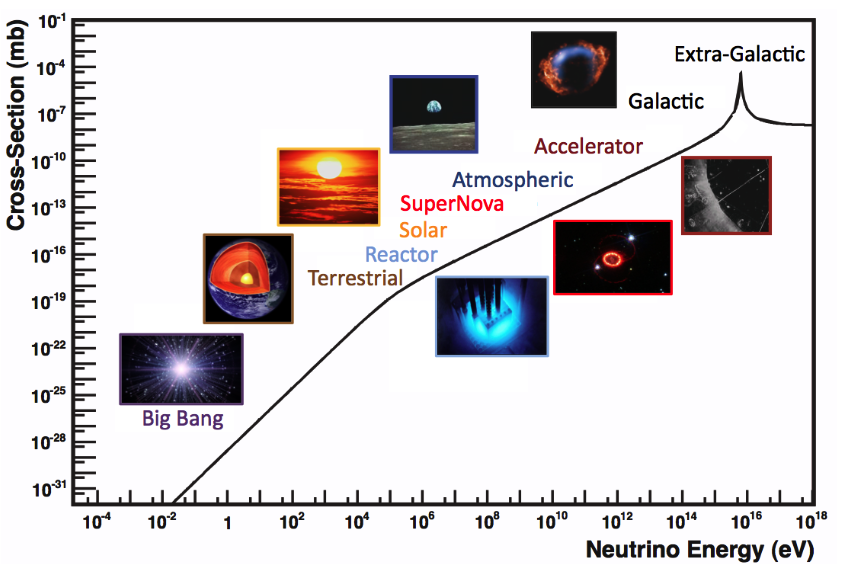
\includegraphics[width=0.8\textwidth]{./sources.PNG}
\caption[Neutrino sources]{Representative figure  of the sources of neutrinos in various energy regimes. Electroweak scattering Cross-section of \nuebar on free electrons as a function of energy is showed as a reference \cite{Formaggio}.}
\label{fig:source}
\end{figure*}

Neutrinos only interact via weak force and gravitational force, they remained obscure for a long time. Even sixty years after their discovery, fascinating properties of neutrinos are still being uncovered. In particular, neutrinos have a very peculiar property called neutrino oscillations that arises from the fact that the flavor eigenstates of neutrinos ( $ \nu_{e}, \nu_{\mu}, \nu_{\tau} $ ) do not coincide with their mass eigenstates ( $ \nu_{1}, \nu_{2}, \nu_{3} $ ). The probability of oscillation depends on propagation distance $L$, neutrino energy $E$ and neutrino mass-squared difference $\Delta m^{2}$. Although absolute masses are not known, we know the two mass-squared difference through oscillation experiments measurements. The current known neutrino data can satisfy two mass hierarchy scenarios, $ \text{m}_{\nu_{1}}<\text{m}_{\nu_{2}}<\text{m}_{\nu_{3}} $ (Normal hierarchy) and $ \text{m}_{\nu_{2}}<\text{m}_{\nu_{1}}<\text{m}_{\nu_{3} }$ (Inverted hierarchy). Figure \ref{fig:hierarchy} shows the hierarchy and fractional content of $ \nu_{e}, \nu_{\mu}, \nu_{\tau} $ in each mass eigenstate.

\begin{figure*}
\centering
  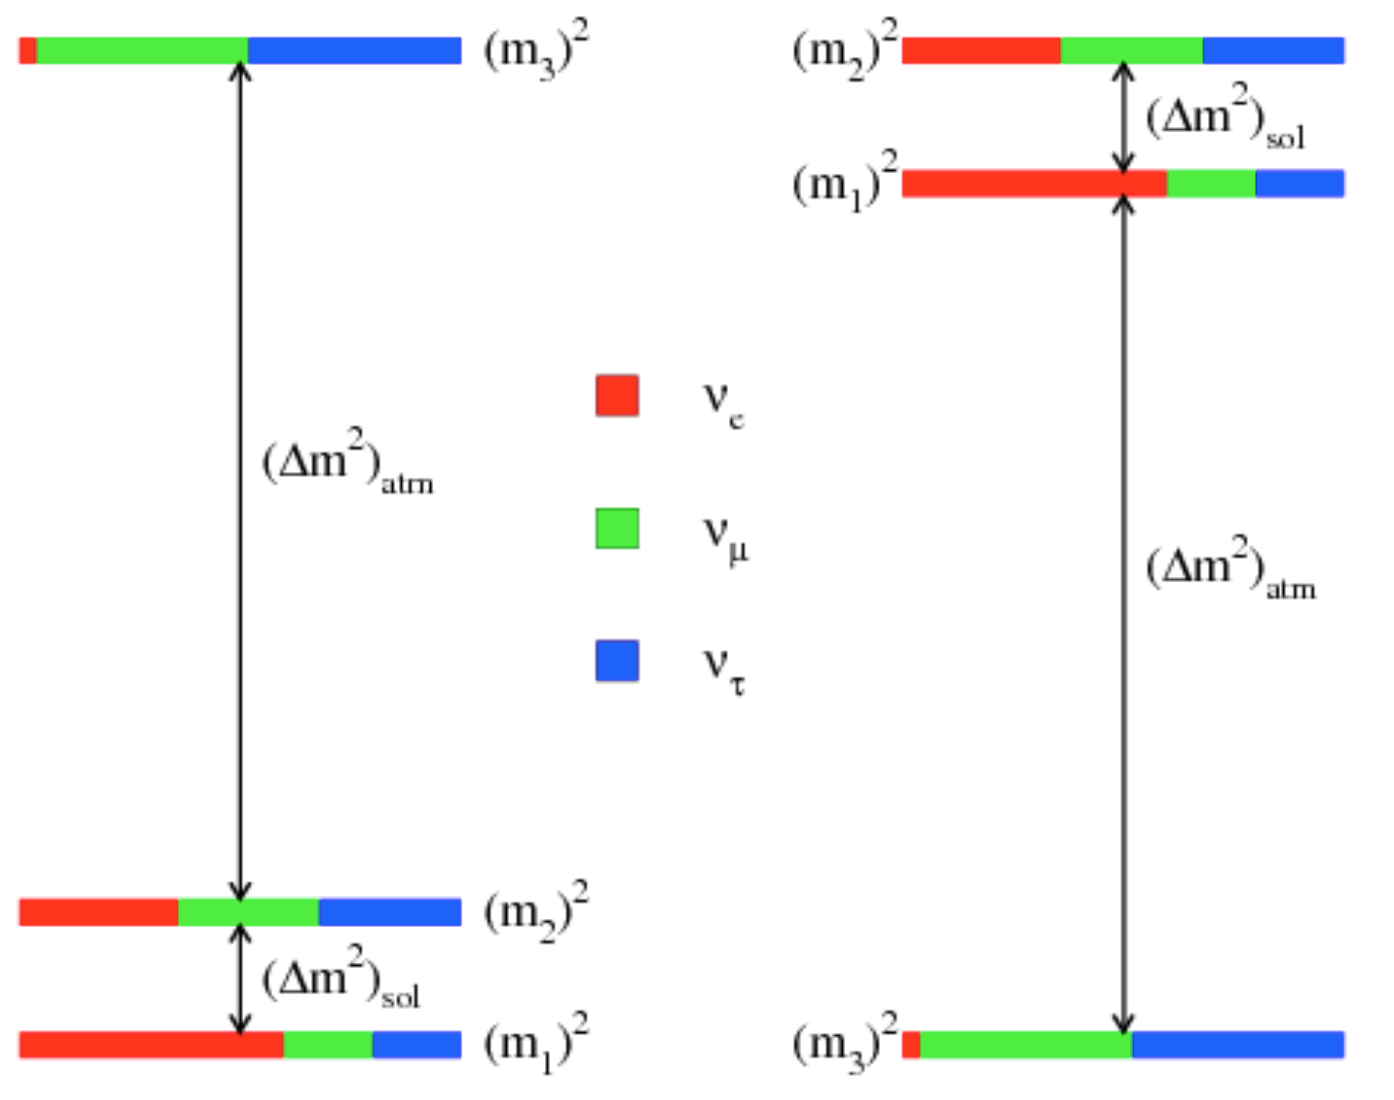
\includegraphics[width=0.4\textwidth]{./hierarchy.PNG}
\caption[Neutrino mass hierarchy]{Illustration of neutrino mass hierarchies for fixed values of mixing angles and $\Delta m^2$. Also shown in color is the fraction of neutrino flavor states in mass eigenstates. \cite{Hewett2012}}
\label{fig:hierarchy}
\end{figure*}

The increasing sensitivity of measuring devices coupled with improvements in experimental techniques led to a very precise understanding of the parameters involved in neutrino oscillations as shown in Table \ref{tab:oscillations}. However, there are still several compelling questions regarding neutrinos that haven't been answered. Some of the questions are, what are the absolute neutrino masses? Where neutrinos get their masses from? Are neutrinos their own antiparticles?  Are there other neutrino species? Is Charge conjugation Parity symmetry (CP) violated in neutrinos? A complete picture of fundamental particles is not possible unless all these questions are answered.


\begin{table}[h]
\centering
\begin{tabular}{ |l | l| }
\hline
  Paramater & Value  \\ \hline
  $\sin ^{2}( \theta_{12})$ & $0.846^{+0.021}_{-0.021}$ \\
  $\sin ^{2}(2 \theta_{13})$ & $0.093 ^{+0.008} _{-0.008}$ \\
  $\sin ^{2}(2 \theta_{23})$ & $0.999^{+0.001}_{-0.018}/ 1.000^{+0.00}_{-0.017} $(normal hierarchy/inverted hierarchy)\\ \hline
  $|\Delta m ^{2} _{atm}|$ & $2.44 ^{+0.06}_{-0.06} / 2.52 ^{+0.07}_{-0.07} \times 10^{-3} \text{eV}^2  $ (normal hierarchy/inverted hierarchy)\\
  $|\Delta m ^{2} _{sol}|$ & $7.53 ^{+0.18}_{-0.18} \times 10^{-5} \text{eV}^2$\\ \hline
\end{tabular}
    \caption[Neutrino oscillation parameters]{Current neutrino oscillation parameters as published by Particle Data Group (PDG) \cite{particle2004particle}}
  \label{tab:oscillations}
  \end{table}

\subsection[Postulation and discovery]{Postulation and discovery of the neutrino}
\label{discovery}
The history of neutrinos can be traced back to the early experiments on radioactivity. During several experiments involving radioactivity via beta decay including those conducted by James Chadwick \cite{chadwick1925xxii}, measurements of the beta spectrum was found to be continuous. Until then, to conserve energy, it is was presumed to be discrete band similar to the spectra from gamma and alpha decays. Further, the nuclear spin of Nitrogen atom, in contradiction to Rutherford's prediction \cite{rasetti1929alternating} of half, turned out to be unity which violated spin conservation. To explain these discrepancies, Wolfgang Pauli \cite{PauliLetter} in 1931, postulated the existence of a spin-half subatomic particle, which he called a \textit{neutron}. He suggested that in beta decay, some of the energy was carried away by this particle and since it is a spin-half particle, it will also account for Nitrogen spin problem. Fermi's theory of beta decay \cite{betaDecay} which assumed the existence of neutrino in beta decay,  added further strong theoretical foundation to this particle. Since an uncharged particle with the name neutron already exists, Fermi in his theory renamed this light uncharged particle \textit{neutrino}. Fermi's theory predicted inverse beta decay with the same strength as neutron decay. 

It was not until 1955 that the neutrino was experimentally discovered by Reines, Cowan and Clyde at the Savannah River reactor in South Carolina \cite{reines1956neutrino}. The reactor provided a very high antineutrino flux of $ 5 \times 10^{13}\textrm{cm}^{-2} \textrm{s}^{-1} $. Antineutrinos from the Savannah River reactor were captured by inverse beta decay on protons in water using
\begin{equation}
 \nuebar + p \rightarrow e^{+} + n .
\end{equation}
The positron from inverse beta decay annihilates with electrons promptly and generates two gammas via
\begin{equation}
e^{+} + e^{-} \rightarrow \gamma + \gamma.
\end{equation}
Gammas thus generated then traveled into a separate scintillation tank, lowered in wavelength and then were collected using photo-multiplier tubes. The neutron from inverse beta decay after thermalizing captures on cadmium:
\begin{equation} 
n + ^{108}Cd \rightarrow \gamma + ^ {109}Cd.
\end{equation}

A delayed time-coincidence was used between the positron and the neutron as a signature of inverse beta decay. The reactor was shut down and reactor-on versus reactor-off data was compared to conclusively prove that the events are indeed from inverse beta decay. Most of the reactor antineutrino experiments to date are performed using a similar method. 

At the time of the discovery of the neutrino, there were two experimentally observed charged lepton counterparts to neutrino, namely the electron and the muon. This raised a question of whether an antineutrino generated in the reaction associated with the electron (from inverse beta decay for example) is the same as the one that is associated with a muon. It was answered at Brookhaven Alternative Gradient Synchrotron(AGS) \cite{danby1962observation} with the use of proton beams. These proton beams hit a Beryllium target at 15 GeV, generating pions which decayed into muons and neutrinos. If these neutrinos could be detected by the same mechanism used for detecting neutrinos associated with electrons, it would indicate that they are not distinct. Since no neutrinos were detected it was concluded that antineutrinos associated with electrons were different from the ones associated with muons. 

Incidentally the answer to whether neutrino is same as its antiparticle was answered by experiment done by Ray Davis \cite{davis1955attempt} in 1955, even prior to the discovery of neutrino. This experiment was performed at Brookhaven Graphite Research Reactor as a source and Carbon Tetrachloride as a target. He attempted to search for neutrinos using
\begin{equation}
 \nuebar +Cl ^{37} \rightarrow e^{-} + Ar^{37}.
\end{equation}

Conservation of lepton number law states that this reaction is not possible. If he did see the conversion of Chlorine-37 to Argon-37, it meant that the neutrino was same as its antiparticle. He did not find evidence of this conversion which indicated that neutrino particle and antiparticle are different from each other.
\subsection[Experimental discoveries]{Experimental discoveries of neutrino properties}
\comment{
Lee and Yang \cite{on1956question} have observed parity violation in Kaon decays and suggested radioactive beta-decay as the test for confirmation. To test this hypothesis, Wu observed an asymmetry in distributions of electrons emitted from $^{60} Co$. Following this discovery, new theories in maximal parity violating Vector-Axial structure of weak interactions were developed by Sudarshan, Marshak(cite) at Harvard and Feynman, Gell-Mann(cite) separately. In 1958, V-A theory was confirmed by Golhaber, Grodzins and Sunyar (cite). This theory predicts that neutrinos are left-handed and antineutrinos are right-handed. }

In 1962, Leon Lederman along with Melvin Schwartz and Jack Steinberger discovered the existence of the muon-neutrino ($ \nu_{\mu}$) at the BNL AGS \cite{danby1962observation}. They used pion beams which decayed to muon and  their associated antineutrinos. These antineutrinos when introduced into spark chamber produced muons but not electrons. It also further led to the idea of individual lepton number conservation. 


An experiment was proposed by Ray Davis Jr. at the Homestake mine \cite{davis1968search} to measure the number of radioisotopes of Argon created when solar neutrinos interacted with Chlorine. During the same time, the Standard Solar Model (SSM) was proposed by John Bahcall \cite{bahcall1964solar} which predicted the neutrino flux from the sun. The neutrino flux predicted in SSM was about three times higher than that observed in the Homestake experiment. This mismatch came to be known as solar neutrino problem.

Bruno Pontecorvo and Vladmir Gribov proposed \cite{gribov1969neutrino} neutrino oscillations as a solution to the solar neutrino problem. They suggested that a neutrino produced in an electron flavor eigenstate has a non-zero probability of being observed in a muon flavor eigenstate. By that time Ziro Maki, Masami Nakagawa and Shoichi Sakata already developed a 2x2 mixing matrix to describe mixing between two flavors of neutrinos \cite{maki1962remarks}. Although the mixing matrix has changed since its inception, it was the first theoretical step in direction of neutrino oscillations. Lacking experimental basis, however, this proposal was not taken seriously. The Homestake experiment ran for over 30 years with many improvements in the detector technology, but the deficiency of neutrino flux was not resolved. Other experiments like the solar neutrino experiment conducted in 1970s by Reines et al.\cite{reines1980evidence} started to favor neutrino oscillation paradigm. Search for neutrino oscillations intensified in the 1990s. Experiments like Soviet-American Gallium Experiment(SAGE) \cite{abdurashitov1994results} , GALlium EXperiment(GALLEX) \cite{hampel1999gallex} and Gallium Neutrino Experiment(GNO) \cite{bellotti2001first} observed $\nu_{e}$ capture on Gallium by
\begin{equation}
\nu_{e} + ^{71}Ga \rightarrow e^{-}+^{71}Ge.
\end{equation}
All these experiments detected neutrinos from the primary proton fusion, $pp$, in the sun and all of them showed a deficiency in solar neutrino flux in low energy range.

In the 1983, Kamioka Nucleon Detection Experiment (KamiokaNDE), a large water Cherenkov detector was built to search for proton decay. Although, no evidence of protons decay was found, the collaboration realized that the detector was sensitive to neutrinos. After upgrades were made, the experiment was named Kamiokande-II and started taking data in 1985. Kamiokande-II found a deficit of solar neutrinos in 4-15 MeV range \cite{hatakeyama1998measurement} which supported the neutrino oscillation hypothesis. To verify the neutrino oscillation hypothesis, Super-Kamiokande(Super-K) experiment, a successor of Kamiokande was built to search for neutrino oscillations by observing solar and atmospheric neutrinos. The first evidence of atmospheric neutrino oscillation was found in 1998 at Super-K \cite{super1999fukuda}. To extend the results from Kamiokande-II, Sudbury Neutrino Observatory  (SNO) was designed to detect solar neutrinos using heavy water as a target. Heavy water has an advantage of being sensitive all the three neutrino flavors. In 2002, SNO provided definitive proof for the neutrino oscillations as the right interpretation for solar neutrino problem \cite{ahmad2002direct}.

Meanwhile, the Direct Observation of Nu Tau(DONUT) collaboration at Fermilab had announced \cite{kodama2001observation} the discovery of tau neutrino, $\nu _{\tau}$, in 2001 giving the standard model its current leptonic picture. The mixing matrix was then extended to include $\nu_\tau$. The mixing matrix was named Pontecorvo-Maki-Nakgawa-Sakata(PMNS) matrix after the scientists that provided the theoretical foundations for it.


\subsection[Role of reactors]{Role of reactors in antineutrino experiments}
\label{reactorrole}

Antineutrinos are produced from a nuclear reactor mainly from fissioning nuclei at a rate of  ~ $10^{20} $ \nuebar$ \textrm{GW}^{-1} \textrm{s}^{-1}$. Almost all of the fissionable reactor fuel ($\sim99.9 \%$) is composed of Uranium and Plutonium isotopes $^{235}$U, $^{238}$U, $  ^{239}\textrm{Pu}$ and $  ^{241}\textrm{Pu}$. They undergo fission via beta decay 
\begin{equation}
n \rightarrow p+e^{-} + \nuebar
\end{equation}
to generate antineutrinos.


\begin{figure*}
\centering
  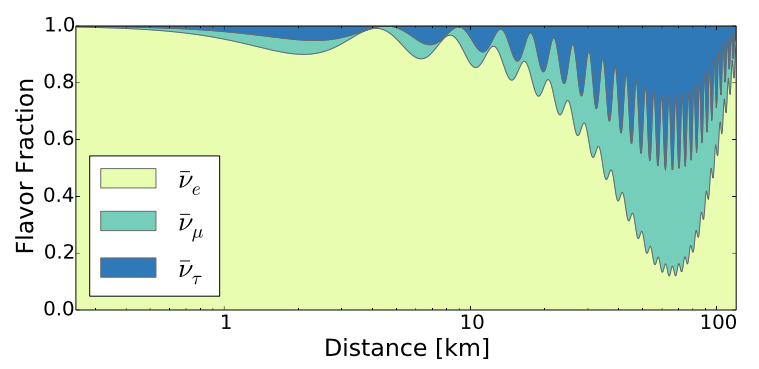
\includegraphics[width=0.8\textwidth]{./Oscillations.PNG}
\caption[Reactor neutrino oscillations]{Illustration of the oscillation of 4 MeV \nuebar as a function of distance based on the current knowledge of oscillation parameters \cite{neutrinoreactorsvogel}.}
\label{fig:oscillations}
\end{figure*}

As shown in Section \ref{discovery}, reactors have historically played a very important role in neutrino physics. Savannah River experiment, a reactor antineutrino experiment was the first to establish the existence of neutrinos. In 1980 Reines et al., \cite{reines1980evidence} while conducting neutrino experiments with heavy water at 11.2 m baseline from reactor, noticed that the ratio of charged versus neutral current interactions was different from the predicted value. This indicated that neutrinos might have an instability as they traversed from origin to their detection. They estimated the oscillation parameters to be in the range $22 ^{\circ} < \theta < 32 ^{\circ} $ with $0.7<\Delta m^2 <1.0$, but emphasized that it was important to perform more experiments to measure the \nuebar spectrum as a function of distance before drawing any conclusions. They also noted that atmospheric and solar neutrino experiments would help identify the phenomenon of oscillations at higher energies. 

These results, in addition to the solar neutrino problem, motivated another reactor antineutrino experiment at Institut Laue-Langevin (ILL), Grenoble called Grenoble Neutrino Oscillation experiment \cite{PhysRevD.24.1097}. They used a segmented detector system with neutron detector sandwiched between cells of liquid scintillator at a distance of 8.5 m from the reactor.  They used a time-delayed coincidence technique and topological cuts in estimating the \nuebar spectrum. Meanwhile, since one of the biggest constraints for reactor antineutrino experiments is the lack of precise absolute \nuebar  spectrum, a beta spectrum measurement of fissile isotopes of $^{235} \textrm{U}$ was made at ILL using a magnetic spectrometer \cite{Schreckenbach1985325}. With an energy binning of 250 KeV, they published the beta spectrum below 9.5 Mev with a precision of 3\%. To date, the beta spectrum measurements made at ILL are used as a standard in modeling reactor antineutrino flux. Grenoble Neutrino Experiment, used the antineutrino flux model from ILL and found that the measured antineutrino spectrum agreed with the beta-converted spectrum from ILL down to the oscillation parameters $\Delta m^{2}= 0.15 \text{eV}^{2}$ for $ \sin ^{2}\theta_{13} = 0.3$. The detector was modified and moved to Switzerland, close to Goesgen reactor, where several measurements were made by shifting the detector to three different locations at the baselines of 37.8 m, 45.9 m and 64.7 m essentially making it a multiple baseline experiment. The multiple baseline approach takes advantage of relative antineutrino spectra to isolate the results from reactor and detector related systematic uncertainties. The measured antineutrino spectrum and rate agreed with the corresponding values predicted by ILL.  



To make a high statistic neutrino spectrum measurement in search for neutrino oscillations, the Bugey experiment was conducted in France near Bugey nuclear power plant in 1980 \cite{kwon1981experimental} and continued in multiple stages until 1995. Bugey used three identical detectors at a baselines of 15 m, 40 m and 95 m from a 2800 Megawatt reactor. Their design consisted of $^{6}$Li loaded liquid scintillator as the target for antineutrinos. Bugey demonstrated that their antineutrino measurements agree with the predictions from the beta spectrum at ILL. In addition, they also placed limits on $\Delta m^{2}$ and $\sin^{2} 2 \theta$ as $ 1 \times10^{-2} eV^{2}$ and $ 2 \times10^{-2}$ \cite{achkar1995search} respectively.

In the 1990s, atmospheric neutrino experiments showed hints of ${\nu}_{\mu}$  oscillations with a large mixing angle $\theta_{23}$ favoring \nuebar disappearance at a long baselines of the order of a km scale. In search for oscillations at this scale, CHOOZ, a reactor antineutrino experiment was setup in France near the CHOOZ power station \cite{apollonio1999limits}. CHOOZ used Gadolinium loaded liquid scintillator as an inverse beta decay target region and a time-delayed coincidence method for background reduction. CHOOZ placed cuts of $\Delta m^{2} > 7 \times 10^{-4} eV^{2}$ for maximal mixing and $\sin^{2} 2 \theta  = 0.1$ for large $\Delta m^{2}$. During the same time, another reactor neutrino experiment called Palo Verde was conducted in Arizona at a distance of 800 m from Palo Verde reactor complex. Palo Verde employed a detector segmentation system similar to Bugey, but much bigger in size and used Gadolinium loaded liquid scintillator as the target region. Palo Verde saw no oscillation \cite{boehm1999palo} in the same parameter space as CHOOZ. 

\begin{figure*}[h]
\centering
\begin{minipage}{.49\textwidth}
  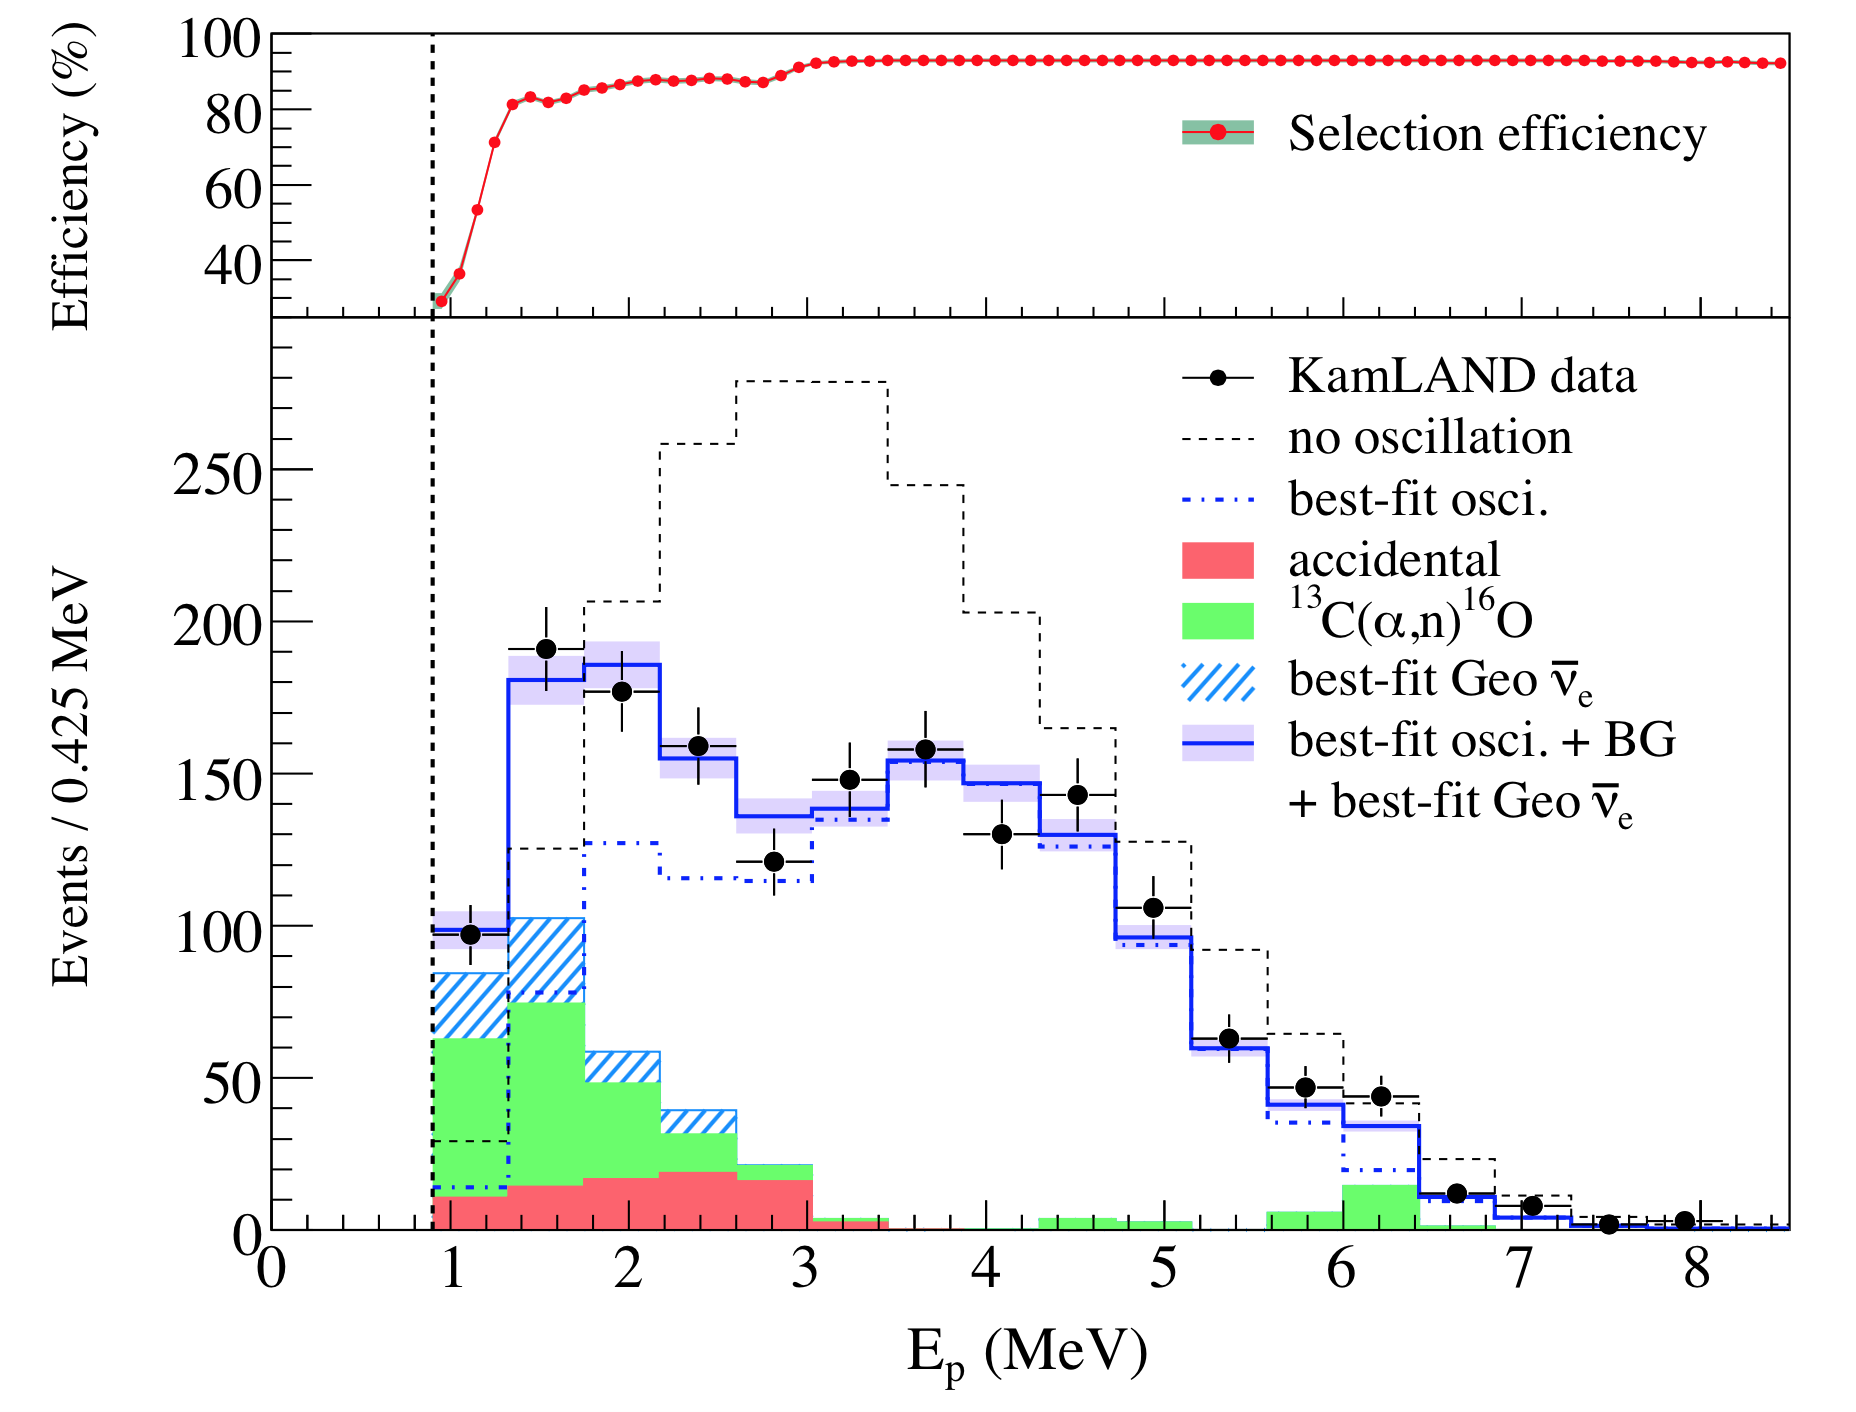
\includegraphics[width=\textwidth]{./KamLAND_Spectrum.PNG}
\end{minipage}
\hfill
\begin{minipage}{.49\textwidth}
  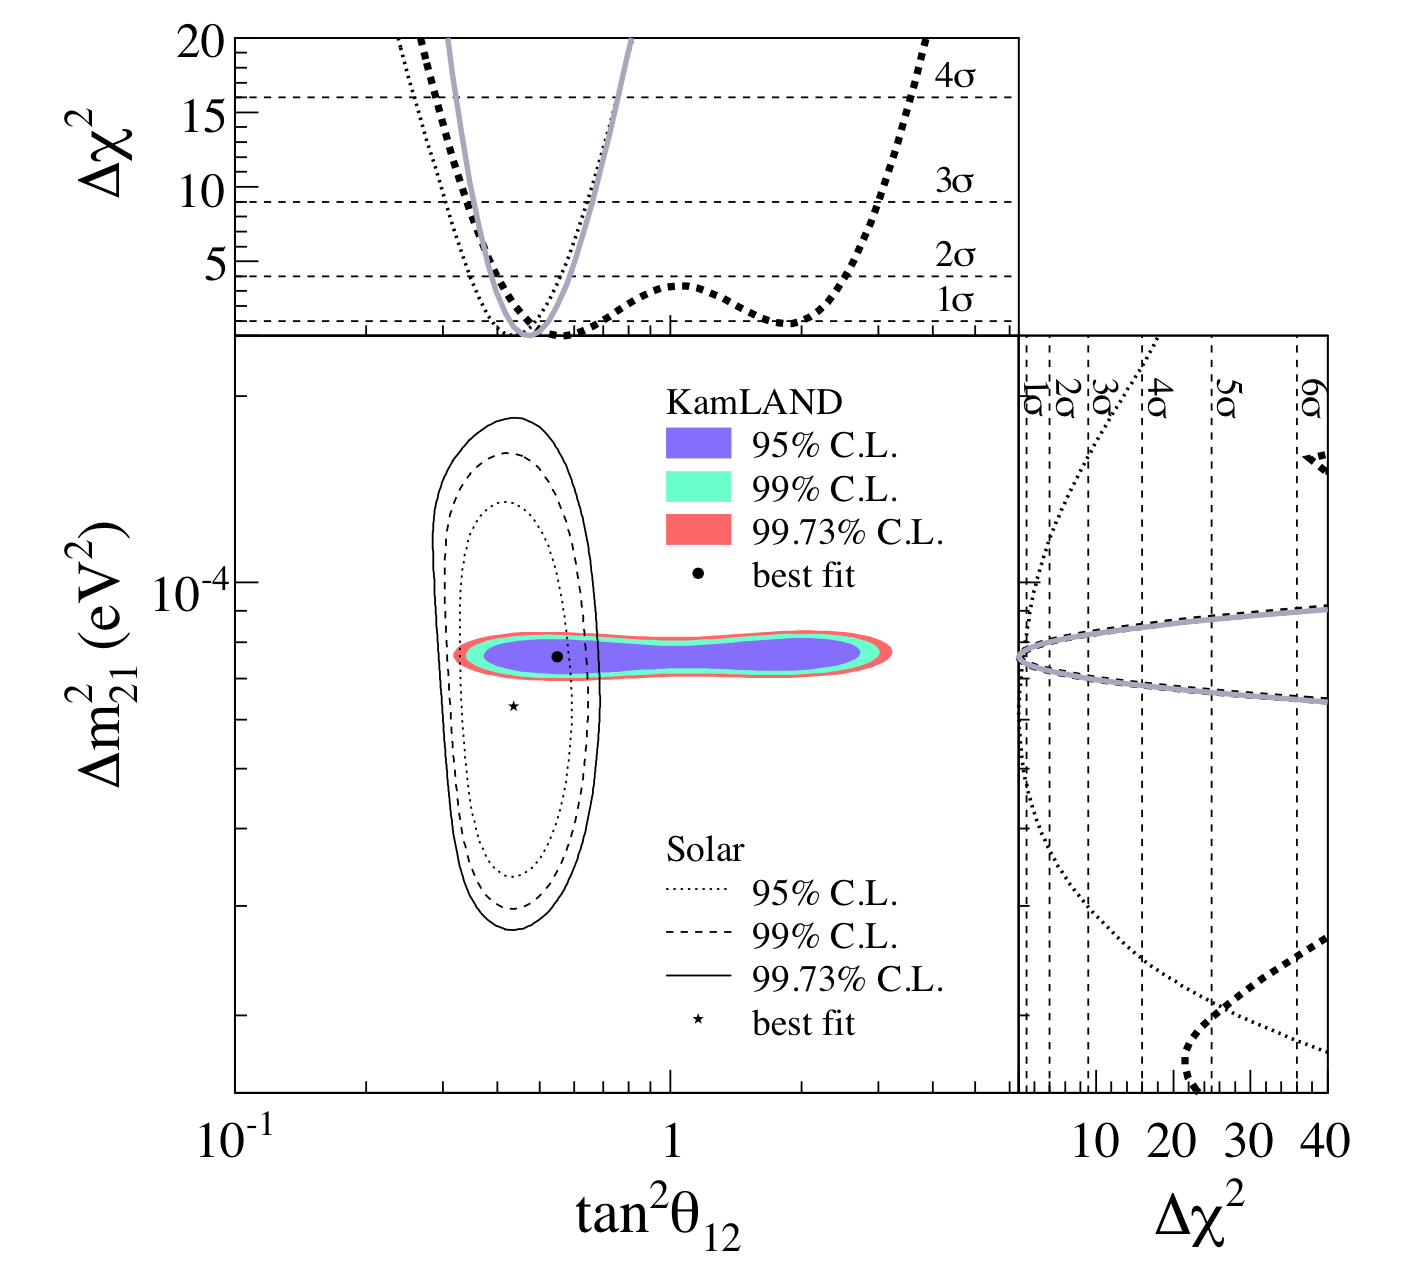
\includegraphics[width=\textwidth]{./KamLAND_Parameters.PNG}
%  \caption{My other caption here}
\end{minipage}

%\includegraphics*[trim=0.1cm 0.1cm 0.1cm 0.1cm, clip=true, width=0.49\textwidth]{./KamLAND_Spectrum.PNG}
%\includegraphics*[trim=0.1cm 0.1cm 0.1cm 0.1cm, clip=true, width=0.49\textwidth]{./KamLAND_Parameters.PNG}
\caption[KamLAND results]{Results from the 2008 report from the KamLAND collaboration \cite{araki2005measurement}. \textit{Left}: The prompt energy spectrum of \nuebar events clearly showing a deviation of data collected from the null oscillation hypothesis case. \textit{Right}: parameter space for $\Delta m^{2}_{12} \text{ and } \tan ^{2} \theta_{12}$, including the best fit parameter.}
\label{fig:KamLAND}
\end{figure*}

A very long baseline antineutrino experiment Kamioka Liquid Scintillator Antineutrino Detector (KamLAND) was built at  at Kamioka \cite{araki2005measurement} to improve the electron-neutrino oscillation parameter space. The detector was surrounded by 53 commercial reactors and is located at a flux-weighted distance of 180 kilometers from those reactors. One kiloton of liquid scintillator was used in the detector and an improved time-delayed coincidence technique between positrons and neutrons was used. The first result reported using 145 days of data showed a deficiency in expected antineutrinos favoring oscillations. In conjunction with solar neutrino data, they showed $ \Delta m^{2}_{21} = 7.9^{+0.6} _{ - 0.5 \times 10^{-5}}$ eV$^2$ and $\tan^{2} \theta_{12} = 0.40 ^{+0.10}_{- 0.07} $ as seen in Figure \ref{fig:KamLAND}. Subsequent results with more data, increased fiducial volume, and reduced systematic uncertainties improved their results. The latest results from KamLAND collaboration were released in 2013 \cite{gando2013reactor} with $ \Delta m^{2}_{21} = 7.53^{+0.18} _{ - 0.18 \times 10^{-5}}$ eV$^2$ and $\tan^{2} \theta_{12} = 0.436 ^{+0.029}_{- 0.025} $ and $\sin ^{2} \theta _{13} = 0.023^{+ 0.002}_{-0.002}$. In addition, they were able to identify the electron neutrino flux of radionuclide sources on earth to be $3.4 ^{+0.8}_{-0.8} \times 10^{6} \text{cm}^{-2} \text{s}^{-1} $ 

Increasing evidence in favor of non-zero value of mixing angle $\theta_{13}$ from accelerator experiments T2K \cite{abe2011indication} and MINOS \cite{Minos} motivated an increased number of multi baseline reactor antineutrino experiments. Meanwhile, Double CHOOZ \cite{DoubleChooz}, a successor to CHOOZ with a single far detector presented its initial measurements of $\sin ^{2} \theta _{13} = 0.086 ^{+ 0.041} _{- 0.041}\text{(stat)} ^{+0.030} _{-0.030}\text{(syst)} $ in 2012.

Daya Bay antineutrino experiment is the first experiment to precisely measure the value of the last mixing angle $\theta_{13}$ in 3-neutrino mixing model. Daya Bay is a neutrino oscillation experiment built near Daya Bay nuclear power station near Shenzhen, China. Daya Bay uses three pairs of commercial low-enriched uranium (LEU) pressurized water reactor cores as source of antineutrinos. Antineutrinos are detected via inverse beta decay(IBD) in Gadolinium loaded liquid scintillator. Daya Bay was able to exclude a $\theta_{13}=$0 at 5.2 $\sigma$ \cite{DayabayZero} with just 52 days of data collection and was able to measure the value of $\sin ^{2}2 \theta_{13} =$ 0.084 $\pm$0.005 \cite{an2013improved} with less than one year of data. Figure \ref{fig:oscillations} shows an illustration of expected composition of flavors of reactor antineutrinos as a function of baseline in a three neutrino model. 

 \begin{figure*}[h]
\centering
  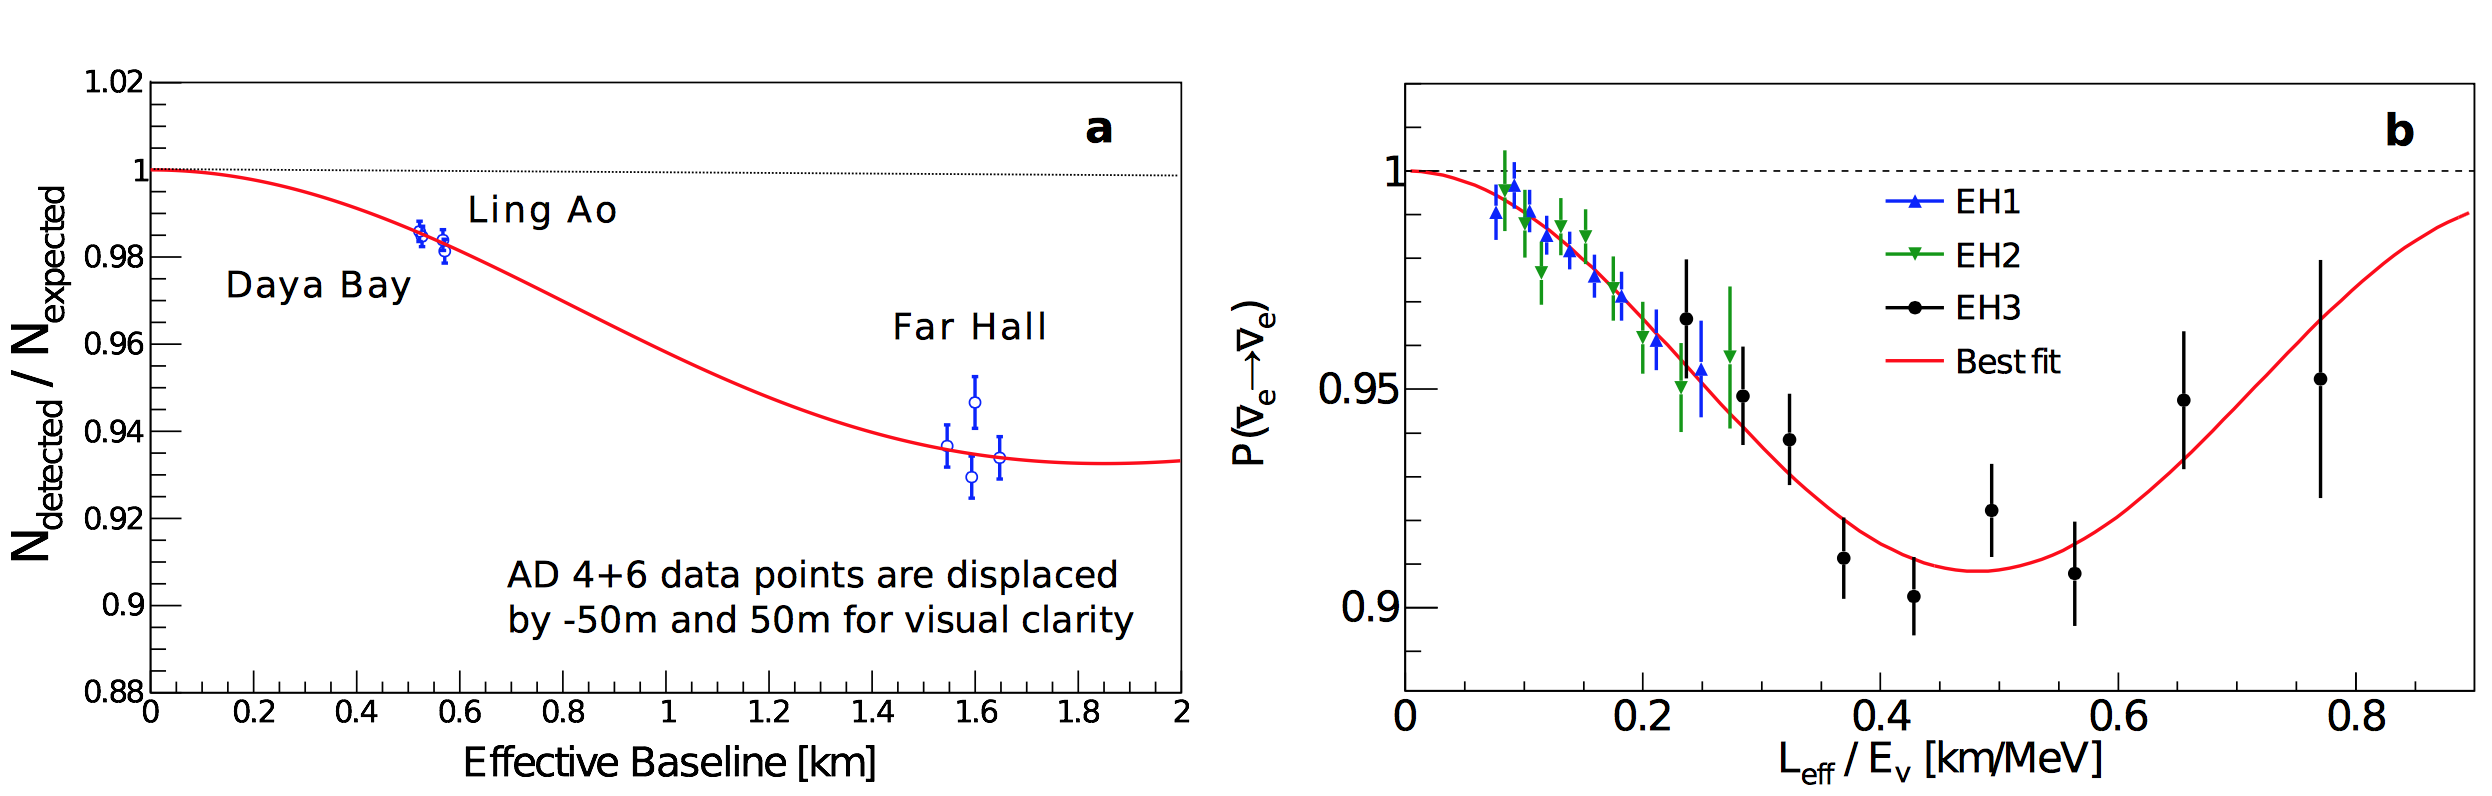
\includegraphics[width=\textwidth]{./Dayabay_Results.PNG}
\caption[Daya Bay results]{Results from Daya Bay collaboration \cite{an2013improved}. Figure \textit{a} shows the ratio of expected flux to observed flux for all of the 8 ADs and the red line is the best fit line. Figure \textit{b} shows the probability of \nuebar being observed as \nuebar as a function of L/E. In both cases, the data points would have fallen on the horizontal dotted line in the null oscillation hypothesis.  }
\label{fig:dayabay_results}
\end{figure*}

\section[Reactor antineutrino anomaly]{Reactor antineutrino anomaly and potential for new physics}
\label{sec:reactoranomaly}
As mentioned above, the antineutrino spectrum calculations made by Schrekenbach et al.\cite{Schreckenbach1985325} have been used as a standard model in reactor neutrino experiments for over 25 years. Thin foils of $^{235}$\textrm{U}, $^{ 238}$\textrm{U} and $ ^{ 239}\textrm{Pu}$  were exposed to thermal neutrons from the ILL reactor. Using a magnetic spectrometer, the beta energy spectrum was measured. Invoking 30 effective(virtual) beta-branches, the measured beta spectrum was converted to antineutrino spectrum. This approach yielded an error of $\sim$3-4\%~ (90\% CL). In a recent paper by Vogel \cite{Vogelconversion}, it was pointed out that because of contribution of thousands of beta branches to the spectrum, the slicing of energy done at ILL is not fine enough to account for all beta branch end points. It was further pointed out that an understanding of average nuclear charge information as a function of their end point energy is needed for precise calculation of antineutrino spectrum. Recently these calculations were revisited in estimating antineutrino spectrum motivated by need for a precise reactor antineutrino spectrum for the Double CHOOZ(far detector only) experiment with improved electron to antineutrino spectrum conversion \cite{2011reactorspectrum}, \cite{mention2011reactor}. The approach was to make an \textit{ab initio} prediction of beta spectrum and to invoke virtual beta branches when there is a mismatch between their prediction and ILL beta spectrum. In addition, a completely \textit{ab initio} approach has been utilized to calculate the contribution due to $^{238}$\textrm{U}. These calculations reported an interaction rate shifted upwards by $\sim$3\% compared to the previous predictions. A complementary work by Huber \cite{Huber} showed that there is a need for an extra term to Fermi theory correction term. Implementing this correction, some old reactor antineutrino experiments located at few tens of meters from the reactor cores were revisited. Although the observed event rates remained same, with a change in the predicted event rates, there is a systematic shift in the ratio of number of the antineutrinos measured versus expected as shown in Figure \ref{fig:reactor_anomaly}. This deficit in observed flux is called the ``Reactor anomaly". 

\begin{figure*}
\centering
  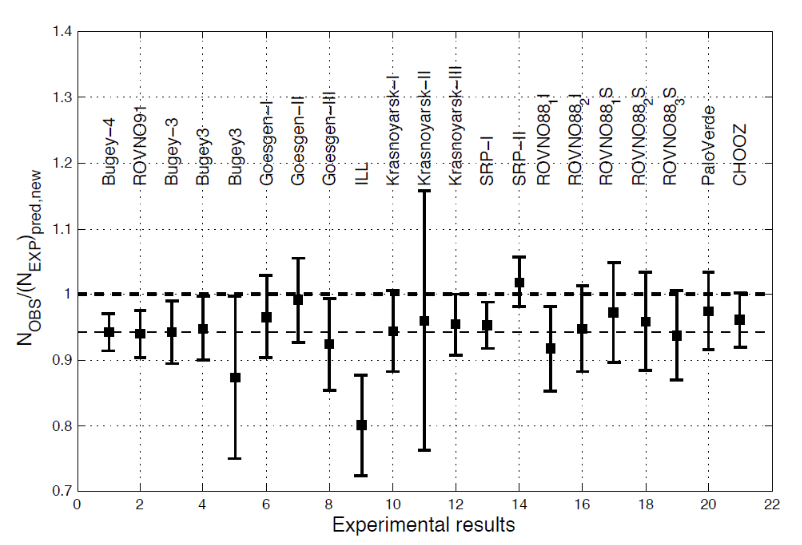
\includegraphics[width=0.8\textwidth]{./Reactor_Anomaly.PNG}
\caption[Reactor antineutrino anomaly]{Ratio of the flux observed versus the new flux prediction for several reactor neutrino experiments.}
\label{fig:reactor_anomaly}
\end{figure*}
A straightforward explanation could be that the previous reactor experiments have been biased in favor of flux measurements to agree with predictions from ILL. But in 2012, Daya Bay published a 5\% deficit in \nuebar from the predicted values. Additionally, Daya Bay and Double CHOOZ reported antineutrino spectra in disagreement with predictions. 

A new flavor of neutrino would be one possible explanations for the discrepancies in the \nuebar flux and spectrum measurement.  This type of neutrino, hence forth referred to as a sterile neutrino($\nu_{s}$) is a neutral lepton which only interacts via gravitational force but has the ability to mix with other flavors of neutrinos. 
\comment{Sterile neutrinos are also a natural explanation for several other discrepancies observed in other neutrino and cosmological experiments(cite).}

The sterile neutrino was hypothesized a long time before the reactor antineutrino anomaly as a possible explanation for the results from Liquid Scintillation Neutrino Detector (LSND). LSND \cite{aguilar2001evidence} was an experiment built at Los Alamos to look for oscillation from a pure $\overline{\nu}_{\mu}$ beam from Los Alamos Meson Physics Facility (LAMPF) to a \nuebar beam. LSND reported an excess in the $\overline{\nu}_{\mu} \rightarrow \nuebar$ appearance channel. This excess indicates the existence of an additional family of neutrinos with $ \Delta \text{m}^{2} \sim 1~ \text{eV}{^2}$ with respect to other three mass states, which can mix with $ \nu_{e}, \nu_{\mu}, \nu_{\tau} $. However, since it has already been established using a precise measurement of Z boson decay that the number of active neutrinos is 2.92 $\pm$ 0.5 \cite{particle2004particle}. This neutrino if exists, has to be sterile, i.e., lacking weak interactions. In a similar L/E parameter space to the LSND analysis, the Mini-Booster Neutrino Experiment (MiniBooNE) experiment \cite{aguilar2007search} also observed an event excess in $\nu_{\mu} \rightarrow \nu_{e}$ and $\overline{\nu}_{\mu} \rightarrow  \overline{\nu}_{e}$. Although, the $\overline{\nu}_{\mu} \rightarrow  \overline{\nu}_{e}$ measurement from the MiniBooNE favors a sterile neutrino in the $ \Delta \text{m}^{2} \sim 1~ \text{eV}{^2}$, the $\nu_{\mu} \rightarrow \nu_{e}$ measurement from the same experiment disfavors it.


\begin{figure*}[h]
\centering
  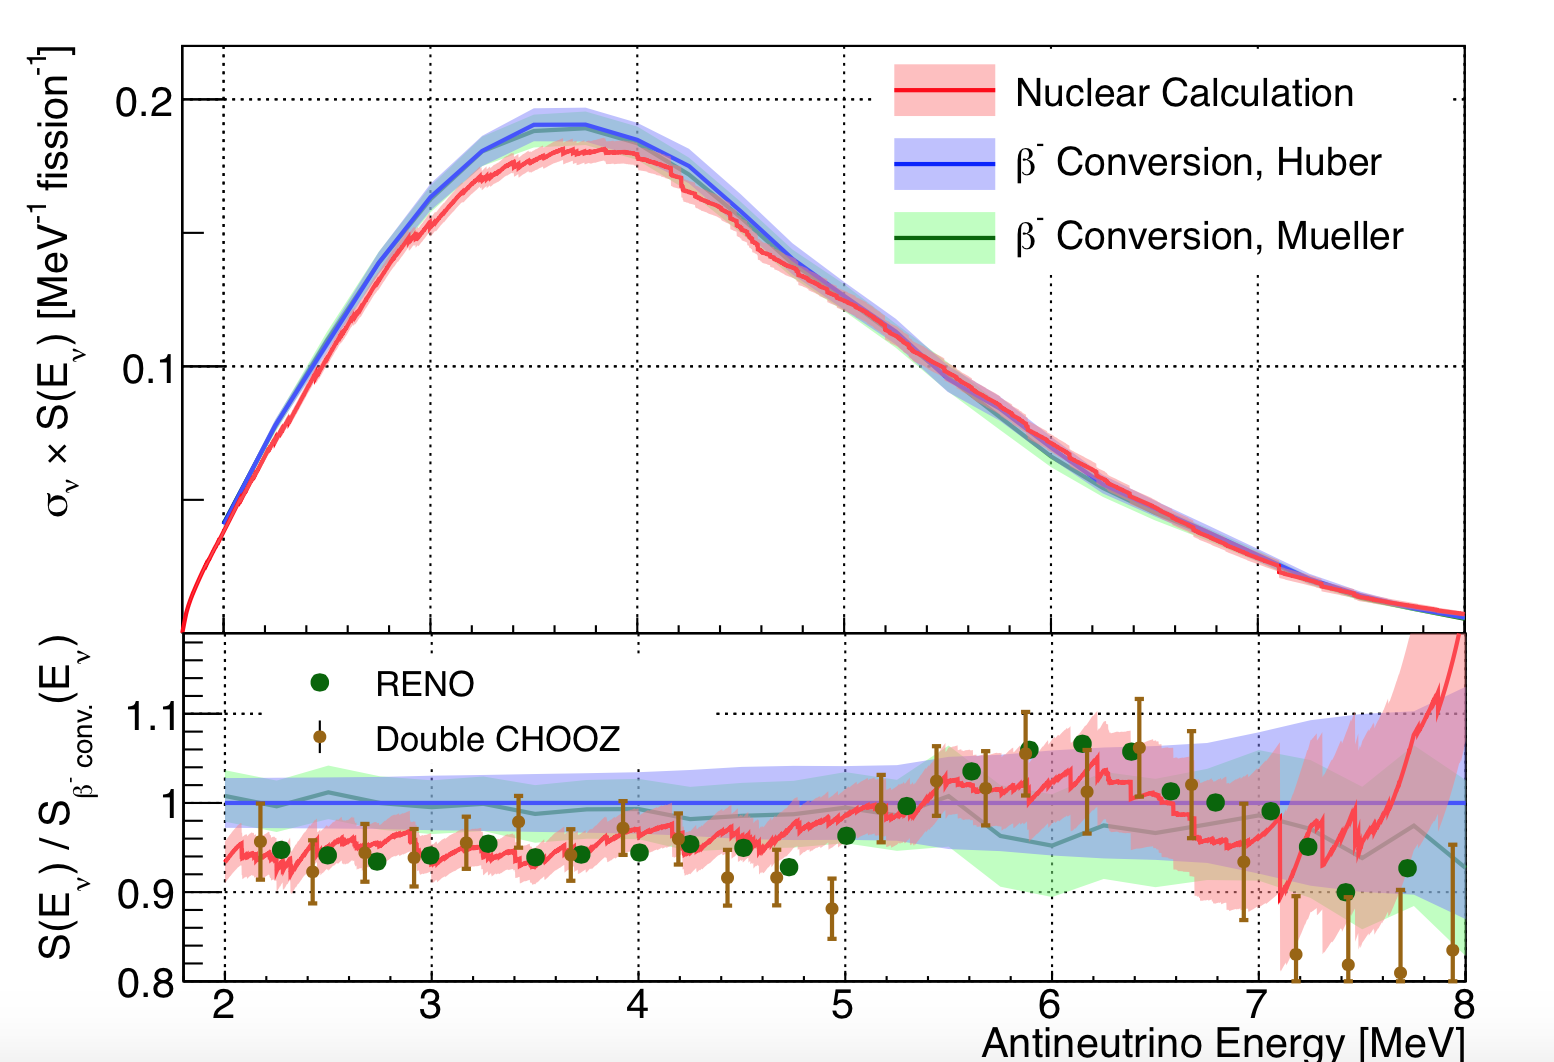
\includegraphics[width=0.6\textwidth]{./DL.PNG}
\caption[Dwyer-Langford spectrum]{The \textit{ab initio} calculation appears in good agreement with RENO and Double CHOOZ \cite{DLSpectrum}. As a comparison other models are shown which disagree with these calculations.}
\label{fig:dl}
\end{figure*}

During calibration measurements, the solar neutrino detectors GALLEX \cite{hampel1999gallex} and SAGE \cite{abdurashitov1994results}, using intense neutrino sources of $^{51} \text{Cr} \text{ and}^{37} \text{ Ar} $, observed an event deficit of $\sim$24\% in the $\nu_{e}$ disappearance channel. This event deficit, referred to as the Gallium anomaly can also be explained using sterile neutrino with a $ \Delta \text{m}^{2} \sim 1~ \text{eV}{^2} $. 

\comment{
In addition, data from the cosmic microwave background favors the existence of an additional degree of freedom which could be a sterile neutrino. The standard cosmological evolution model favors this neutrino to be $ \Delta \text{m}^{2} \sim 1~ \text{eV}{^2}$ .
}

Although there is evidence in favor of a sterile neutrino at $ \Delta \text{m}^{2} \sim 1~ \text{eV}{^2}$, there are other possible theories that can explain above anomalies independently. Here, attention is given only to the reactor anomaly. The reactor anomaly could be explained by experimental systematic uncertainties. It could also be caused by lack of theoretical understanding of the underlying nuclear physics. It was remarked in a recent work \cite{Hayes2013}, that the uncertainties in the analysis of the reactor anomaly that arises from structure of forbidden transitions are too high to infer an anomaly. More recently, an \textit{ab initio} antineutrino calculation \cite{DLSpectrum} made using Evaluated Nuclear Structure Data File (ENSDF) data \cite{ensdf2003online} agree with spectrum from  RENO and Double CHOOZ. As such, the accuracy of ILL beta spectrum measurements has been questioned. Experiments that have the ability to prove or disprove the sterile neutrino hypothesis as well as to provide a deeper understanding of the reactor antineutrino spectrum are needed to better understand these anomalies. 


\section[Phenomenology]{Phenomenology}

\subsection[Neutrinos and neutrino oscillations]{Neutrinos and neutrino oscillations}
Neutrinos are very different from other particles in the standard model. As already mentioned, because of the misalignment between neutrino mass and flavor eigenstates, neutrinos undergo a phenomenon called oscillation.
For demonstration, the Lagrangian involving charged current neutrino interactions with leptons can be written as 

\begin{equation} \mathcal{L} = \frac{-g}{2 \sqrt{2}} \sum\limits_{\alpha , i} [\overline{l}_{\alpha} \gamma^{\mu}(1-\gamma_{5})\nu_{i} W^{-}_{\mu} + \overline{\nu}_{i} \gamma^{\mu}(1-\gamma_{5})l_{\alpha} W^{+}_{\mu}].
\end{equation}
Where, $g$ is the weak coupling constant, $\alpha = e,\mu,\tau$ are the flavor eigenstates, $i=1, 2, 3$ are the mass eigenstates, $l$ stands for any lepton, $\nu$ for any neutrino and $W^{\pm}$ stand for the W Bosons. This Lagrangian can also be written in the neutrino mass eigenbasis as, 
\begin{equation} \mathcal{L} = \frac{-g}{2 \sqrt{2}} \sum\limits_{\alpha , i} [\overline{l}_{\alpha} \gamma^{\mu}(1-\gamma_{5})U_{\alpha i}\nu_{i} W^{-}_{\mu} + \overline{\nu}_{i} \gamma^{\mu}(1-\gamma_{5})U^{*}_{\alpha i}l_{\alpha} W^{+}_{\mu}].
\end{equation}
 Where, $U_{\alpha i}$ is a unitary matrix that transforms mass eigenbasis to flavor eigenbasis. This matrix is called Pontecorvo-Maki-Nakagawa-Sakata(PMNS) matrix and can be written as 
 \begin{equation}
U_{PMNS} = \begin{pmatrix}
U_{e1} & U_{e2} & U_{e3} \\
U_{\mu 1} & U_{\mu 2} & U_{\mu3} \\
U_{\tau 1} & U_{\tau 2} & U_{\tau 3} 
     \end{pmatrix}
\end{equation}
For the sake of convenience, this matrix was historically divided into several pieces in terms of their mixing angles and has been used as
\begin{align}
U_{PMNS} =
\begin{pmatrix}
1 &  & \\
 & \cos{\theta_{23}}& \sin{\theta_{23}}\\
 &  - \sin{\theta_{23}} & \cos{\theta_{23}} 
\end{pmatrix}
\begin{pmatrix}
\cos{\theta_{13}}&  & \sin{\theta_{13}} e^{-i \delta} \\
& 1& \\
- \sin{\theta_{13}} e^{-i \delta}&  & \cos{\theta_{13}} 
\end{pmatrix}
\begin{pmatrix}
\cos{\theta_{12}}&& \sin{\theta_{12}}  \\
- \sin{\theta_{12}} &  & \cos{\theta_{12}} \\
& 1&
\end{pmatrix} \nonumber \\
\begin{pmatrix}
e^{i\xi_{1}/2}&&   \\
 & e^{i\xi_{2}/2}  &  \\
& &1
\end{pmatrix}
\end{align}
where $\theta \text{s}$ stand for different mixing angles, $\delta$ is the CP violating phase, $\eta_{1} \text{ and } \eta_{2}$ are Majorana mass terms. 
According to this matrix, a neutrino produced in one flavor eigenstate, after traveling some distance in vacuum has a non-zero probability of being observed in a different flavor eigenstate, given by 
\begin{equation} P(\nu_{\alpha} \rightarrow \nu_{\beta})=\delta_{\alpha, \beta}-4 \sum\limits_{i>j} \text{Re}(U^{*}_{\alpha i} U_{\beta i}U_{\alpha j}U^{*}_{\beta j})  \sin^{2}(\frac{\Delta m^{2}_{ij} L}{4 E}) +2 \sum\limits_{i>j} \text{Im}(U^{*}_{\alpha i} U_{\beta i}U_{\alpha j}U^{*}_{\beta j}) \sin(\frac{\Delta m^{2}_{ij} L}{2 E}) .
\end{equation}
Where $\Delta m^{2}_{ij}=m^{2}_{i}-m^{2}_{j}$, L is the neutrino path length and E is the energy of the neutrino. It is important to note that P($\nu_{\alpha} \rightarrow \nu_{\beta}$) is non-zero only when $\Delta m^{2}_{ij}$ is non-zero. This implies that observation of oscillation between two flavors is proof that at least one neutrino must have non-zero mass. By tuning the values of L and E, several terms in the equation can be made dominant often making the oscillation probability a two neutrino oscillation approximation,
\begin{equation}
 P(\nu_{\alpha} \rightarrow \nu_{\beta})\simeq\sin^{2}2\theta_{\alpha \beta} \sin^{2}(\frac{\Delta m^{2} L}{4 E}) .
 \end{equation}
In fact, most neutrino detectors exploit this approximation to search for neutrino oscillations with a great precision. Consequently, the survival probability can be written as 
\begin{equation} 
P(\nu_{\alpha} \rightarrow \nu_{\alpha}) \simeq 1-\sin^{2}2\theta \sin^{2}(\frac{\Delta m^{2} L}{4 E}) 
\end{equation}
In case of reactor neutrino experiments measuring the disappearance of \nuebar, the survival probability of \nuebar can be written as 
\begin{equation}
\label{eq:theta13}
 P(\nuebar \rightarrow \nuebar)\simeq\sin^{2}2\theta_{13} \sin^{2}(\frac{\Delta m^{2}_{13} L}{4 E}) .
 \end{equation}
Additional corrections should be made for neutrinos traveling in matter because of forward scattering, but for very small distances of a few meters, it can be neglected. Reactor neutrino experiments like Daya Bay, Double CHOOZ and RENO used this equation \ref{eq:theta13} to measure $\theta_{13}$.

\subsection[Reactor neutrinos]{Reactor neutrinos}
Most of the neutrino experiments use the IBD reaction to measure the \nuebar spectrum. In such an experiment, neutrino oscillation parameters can be obtained by comparing the observed antineutrino spectrum to the equation,

\begin{figure*}[h]
\centering
  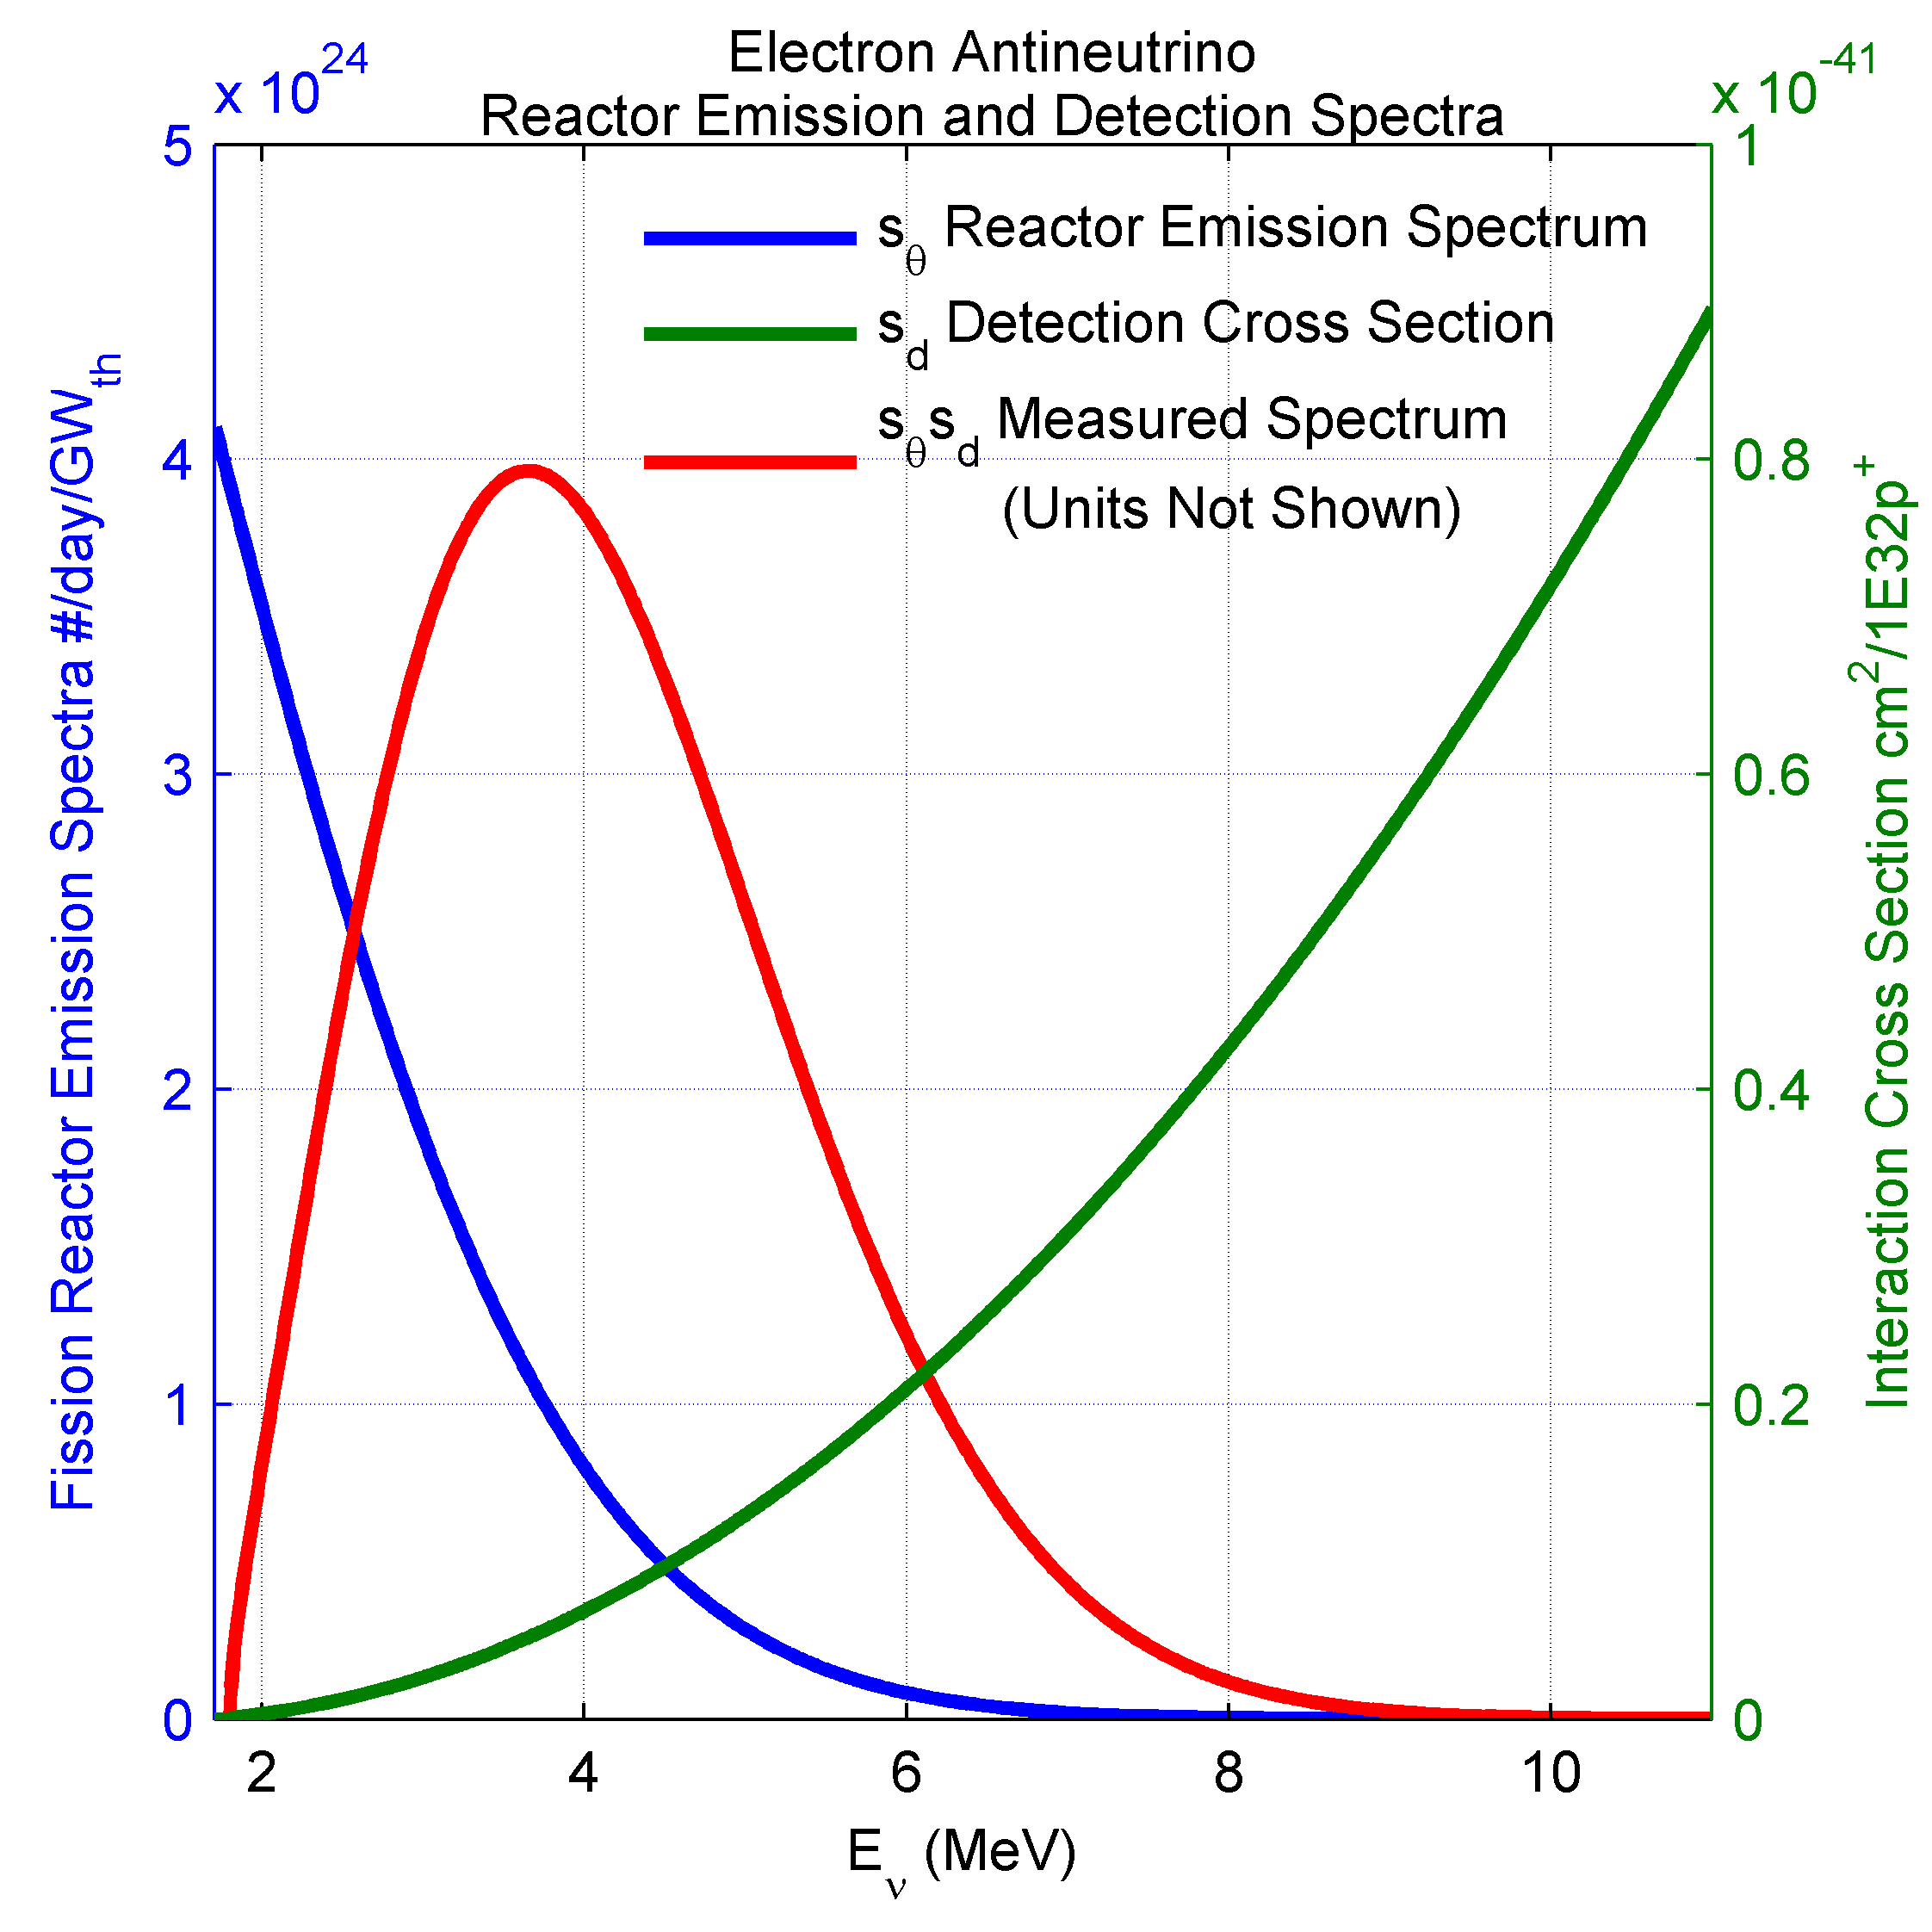
\includegraphics[width=0.45\textwidth]{./spectrum.png}
\caption[Reactor antineutrino spectrum at detector]{An illustration of measured antineutrino spectrum at a detector as a function of energy. It can be obtained by taking product of  the inverse beta decay cross-section($\sigma (E_{\nu_{e}})$) and reactor antineutrino emission spectrum ($S_{\text{tot}}(E_{\nu_{e}})$). For simplicity, oscillations are suppressed in this figure\cite{Jocher2013131}.}
\label{fig:antinuSpectrum}
\end{figure*}

\begin{equation}
\label{eq:obsspectrum}
\frac{dn_{\nu}}{d E_{\nu}}= N_{p} \eta(E_{\nu}) \sigma(E_{\nu}) \frac{P_{ee}(E_{\nu},L)}{4 \pi L^{2}}S_{\text{tot}}(E_{\nuebar}),
\end{equation}
where $N_{P} $ is the number of target protons, $ \eta(E_{\nu}) $ is the energy-dependent detector efficiency, $\sigma (E_{\nu})$ is the energy-dependent IBD cross-section, $ P_{ee}$ is the \nuebar survival probability and $ S_{\text{tot}}(E_{\nuebar})$ is the antineutrino spectrum emitted by reactors is given by 
\begin{equation}
S_{\text{tot}}(E_{\nuebar}) = \sum_{k} f_{k} S_{k}(E_{\nuebar}).
\end{equation}
Here, $f_{k}$ corresponds to the contribution of fission nuclei to total number of fissions of $k_{th}$ branch and $S_k$ is the corresponding antineutrino spectrum. The antineutrino spectrum for each branch is weighted sum of the contributions through various $\beta$ decay chains of its fission products. In principle, an \textit{ab inito} calculation using all the $\beta$ chains would provide a perfect antineutrino spectrum. Lack of information of several nuclei $\beta$ decay chains and systematic errors in nuclear calculations leads to over $10 \%$ uncertainty in antineutrino spectrum using an \textit{ab initio} calculation. 
To overcome this issue, a $\beta$ spectrum measurement was done on nuclear isotopes at ILL. Using energy conservation equation 
\begin{equation}
\label{eq:enuconversion}
E_{e} + E_{\nu}=E_{0},
\end{equation}
 this beta spectrum can be converted to antineutrino spectrum. However, that needs information of the contributions of all beta branches of ILL spectra which is not available. So, a conversion protocol was developed \cite{Schreckenbach1985325} using 30``virtual" $\beta$ branches. The $\beta$ spectrum of virtual branch was taken to be 
\begin{equation}
\label{eq:virtual}
S_{virtual}(Z, A, E_{e}) = K \times \mathscr{F}(Z, A, E_{e}) \times p_{e} E_{e} (E_{e}-E_{0})^{2}\times C(E_{0}) \times (1+ \delta (Z, A, E_{e})),
\end{equation}
where $K$ is to account for normalization, $\mathscr{F}$ is the Fermi function, $p_{e} E_{e} (E_{e}-E_{0})^{2}$ accounts for phase space, $C(E_{0})$ is the a term included to account for forbidenness in transition, the final term $(1+ \delta (Z, A, E_{e}))$ is a correction term where $Z$ and $A$ are the charge and the atomic number of parent nuclei respectively. $Z$ dependence on $E_{0}$ from the observation of nuclear databases was taken to be 
\begin{equation}
Z(E_{0}) \simeq 49.5 - 0.7 E_{0} - 0.09 E^{2}_{0}, Z \leq 34.
\end{equation}
The spectrum from Equation \ref{eq:virtual} was fit to measured beta spectrum and, using Equation \ref{eq:enuconversion} was converted to antineutrino spectrum. After conversion, a weak magnetism correction and a finite coulomb correction is incorporated by 
\begin{equation}
\Delta S_{branch}(E_{\nu}) = 0.65(E_{\nu} -4.00) \%.
\end{equation}
In addition to the $\beta$ conversion method, a purely analytical approximation \cite{vogel1989neutrino} is often used for practical purposes which is given by 
\begin{equation}
\frac{dN_{\nu}}{dE_{\nu}}=\text{exp}(a_{0}+a_{1} E_{\nu} + a_{2} E^{2}_{\nu}).
\end{equation}
In 2011, in the context of single detector neutrino oscillation measurement for Double CHOOZ experiment, the antineutrino spectrum measurement was improved. Information from the nuclear database ENSDF \cite{ensdf2003online} and pandemonium corrected $\beta$ branches, wherever applicable was used to make $\beta$ spectrum calculations. To match the ILL $\beta$ spectrum, the missing contribution was fit using 5 virtual $\beta$ branches with $Z=56$. The antineutrino spectrum obtained this was turned out to be $\sim$3$\%$ higher than ILL antineutrino spectrum thus leading to ``Reactor anomaly".

\subsection[Sterile neutrino]{Sterile neutrino}
A sterile neutrino is a weak singlet that does not take part in weak interactions. It can mix with other active i.e, weakly interacting neutrinos and it may have Yukawa interactions involving Higgs boson. A sterile neutrino is one of the most straight forward explanations of the anomalies described in \ref{sec:reactoranomaly}. The simplest hypothesis is a 3+1 (3 weakly interacting neutrinos + 1 sterile neutrino) neutrino model.
 \begin{figure}[h]
\centering
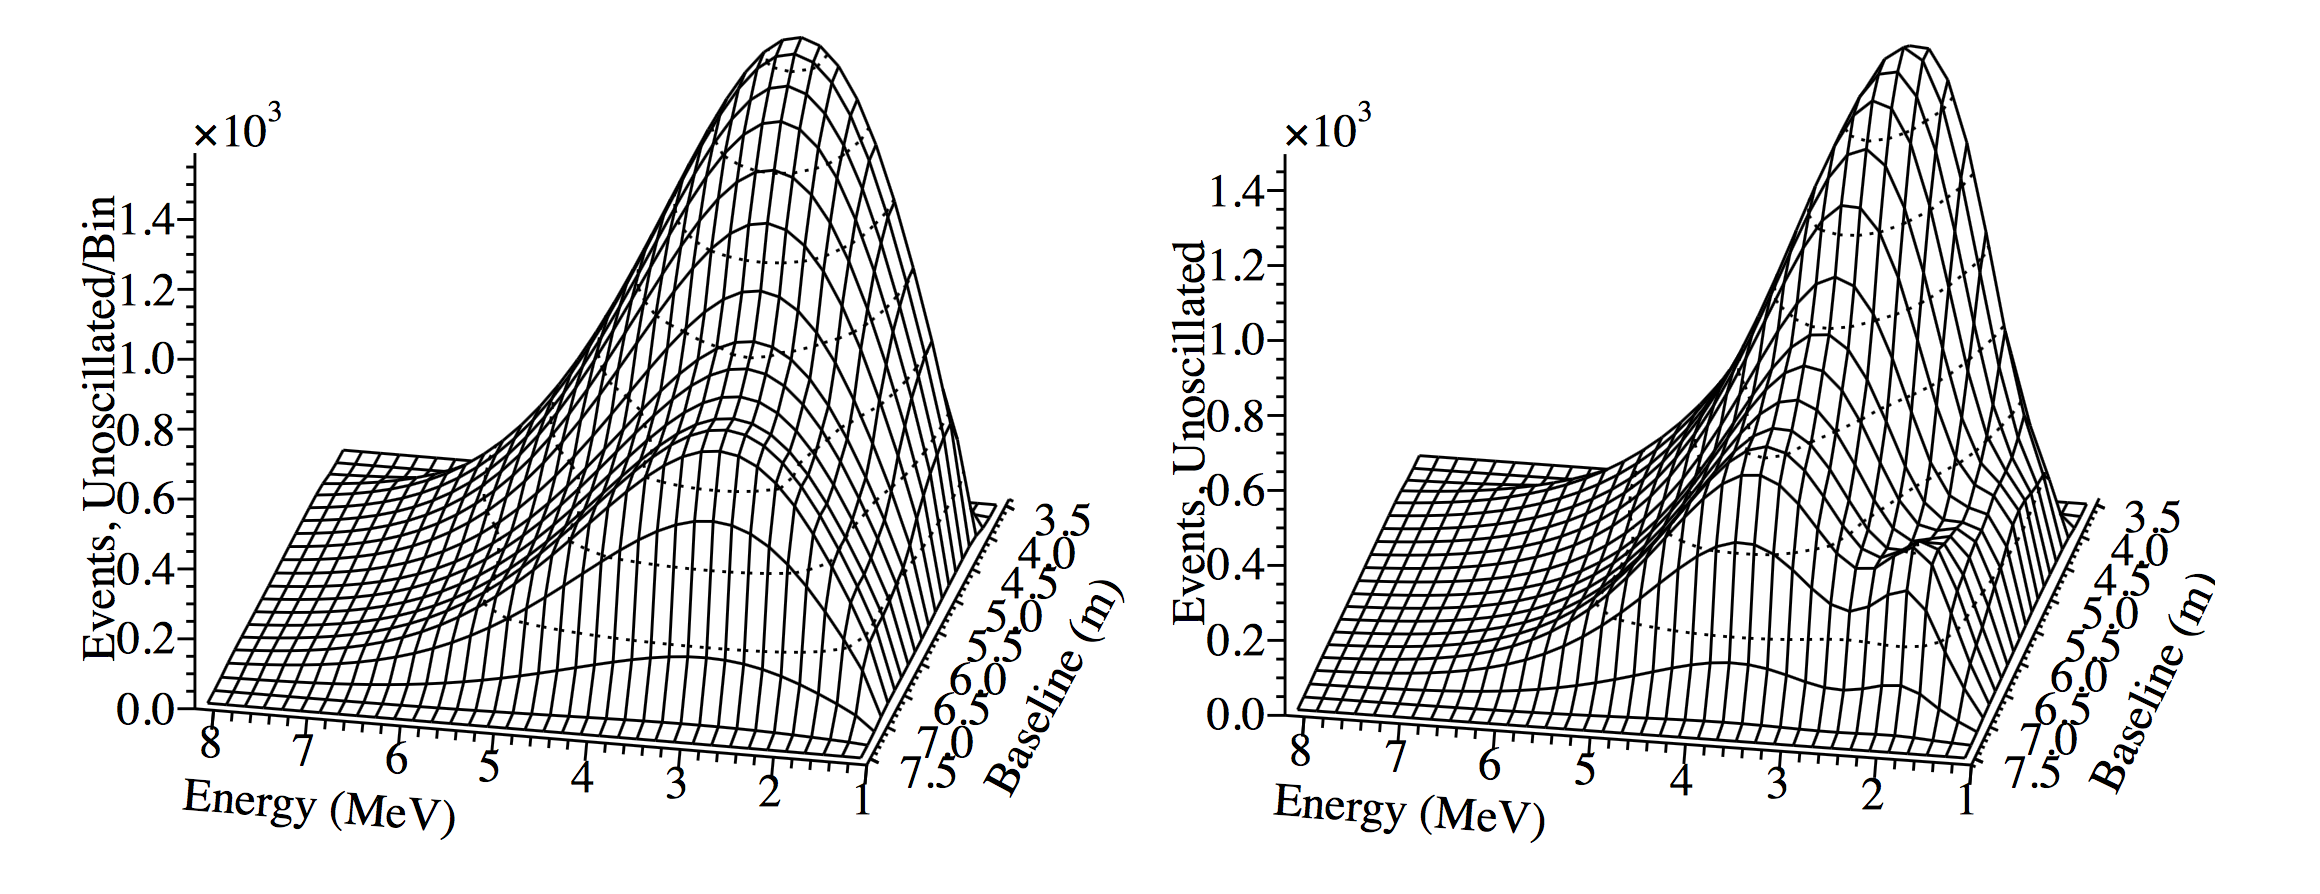
\includegraphics[width=\textwidth]{./SterileOscillation.PNG}
\caption[Sterile neutrino oscillations]{A comparison between detected neutrinos for unoscillated(left) and oscillated(right) cases in a reactor \nuebar detector for $\Delta m^{2} = 1.8 \text{eV}, \sin^{2}2\theta_{ee}=0.5$  and with a $3 \times 1 \times 1$ m detector and 20 MW reactor power.}
\label{fig:sterileOscillation}
\end{figure}
To include the sterile neutrino, the PMNS matrix can be extended and written as
 \begin{equation}
U = \begin{pmatrix}
U_{e1} & U_{e2} & U_{e3} & U_{e4} \\
U_{\mu 1} & U_{\mu 2} & U_{\mu3}  & U_{\mu 4}\\
U_{\tau 1} & U_{\tau 2} & U_{\tau 3}  & U_{\tau4} \\
 U_{s 1} & U_{s 2} & U_{s 3}  & U_{s4}
     \end{pmatrix}
\end{equation}
Using the matrix, the effective flavor transition probability in a short baseline neutrino experiment for a 3+1 model is given by 
\begin{equation}
P(\nu_{\alpha} \rightarrow \nu_{\beta}) \simeq \sin^{2} 2 \theta _{\alpha \beta} \sin^{2}(\frac{\Delta m^{2}_{41} L }{4 E}),
\end{equation}
where $\alpha, \beta = e, \mu, \tau, s $ and $\alpha \neq \beta$, where $s$ stands the sterile neutrino. The amplitude of transition is given by 
\begin{equation}
\sin^{2} 2 \theta _{\alpha \beta} \simeq 4|U_{\alpha 4}|^{2}|U_{\beta 4}|^2,
\end{equation}
\begin{equation}
\sin^{2} 2 \theta _{\alpha \alpha} \simeq 4|U_{\alpha 4}|^{2}(1- |U_{\alpha 4}|^2).
\end{equation}
In case of a short baseline reactor experiment the survival probability of \nuebar can be written as 
\begin{equation}
\label{eq:eemixing}
P(\nu_{e} \rightarrow \nu_{e}) \simeq 1- \sin^{2} 2 \theta _{ee} \sin^{2}(\frac{\Delta m^{2}_{41} L }{4 E}).
\end{equation}	
Figure \ref{fig:sterileOscillation} shows the effect of mixing in sterile neutrinos as a function of baselines and energy of neutrinos.  

\section[PROSPECT experiment]{PROSPECT experiment}

The Precision Reactor Oscillation and SPECTrum(PROSPECT) experiment is a US-based very short baseline antineutrino experiment \cite{PROSPECT}. This experiment aims to detect reactor antineutrinos emitted from the High Flux Isotope Reactor(HFIR), a highly enriched uranium(HEU) nuclear reactor located at Oak Ridge National Laboratory(ORNL). It is a multiphase experiment where Phase-I consists of near detector (Prospect-2ton) at $\sim$7-10~m from the reactor and Phase-II consists of a near and a far detector $\sim$20~m from the reactor. Lithium-loaded liquid scintillator is used as the target in the detector to enhance detection efficiency. 
PROSPECT utilizes IBD reaction to the measure flux and energy spectrum of reactor $\nuebar$. 
An antineutrino from the reactor interacts with a proton in the proton-rich liquid scintillator and produces a positron and a neutron :

\begin{equation}
\nuebar + p \rightarrow e^{+}+n.
\end{equation}

The positron annihilates with an electron in the detector and produces two gammas(also called prompt signal) which are detected using photomultiplier tubes(PMT)

\begin{equation}
e^{+} + e^{-} \rightarrow \gamma + \gamma .
\end{equation} 

The second product of the IBD,  the neutron thermalizes by scattering with several protons in the liquid scintillator and captures on Lithium-6 (also called delayed signal) to give rise to tritium and alpha particle with specific energies of 2.05 MeV and 2.75 MeV respectively. 

\begin{equation}
\label{eq:licapture}
n + ^6 Li \rightarrow \alpha + _1^3 H .
\end{equation} 

Both tritium  and alpha deposit their energy almost instantaneously which is also detected by PMTs. The time separation between triggers from positrons and neutrons has a typical signature of $ < 100 \mu$s and provides a time-coincidence that can be used to reject uncorrelated background events. This, in addition to pulse shape discrimination provides good background rejection capabilities.

\subsection[Physics goals]{Physics goals of PROSPECT experiment}

\begin{table}[h]
\centering
    \begin{tabular}{|l | l | l |} \hline
      \multicolumn{2}{|c|}{Parameter} & Value\\ \hline
      \multirow{4}{*}{Reactor} & Power & 85 MW \\
      & Shape & cylindrical  \\
      & Radius & 0.2~m \\
      & Height & 0.3~m \\
      & Fuel & HEU \\
      & Duty cycle & 41\% reactor-on \\ \hline
      \multirow{8}{*}{Detector} & Cross-section (near) & 1.0~m$\times$1.5~m \\
      & Cross-section (far) & 1.0~m$\times$3.0~m \\
      & Baseline coverage (near) & 2.1~m \\
      & Baseline coverage (far) & 4.2~m \\
      & Efficiency & 30\%  \\  
      & Proton density & 5.5$\times$10$^{28}\frac{p}{m^3}$ \\
      & Position resolution & 15~cm   \\
      & Energy resolution & 4.5\%/$\sqrt{E}$ \\ \hline
      \multirow{2}{*}{Background}& S:B ratio & 1 \\
      & Background shape & 1/E$^2$ + Flat \\ \hline
      \multirow{3}{*}{Other} & Run Time & 1 or 3 calendar years  \\
      & Closest distance (near) & $\sim$7m \\ 
      & Closest distance (far) & $\sim$15m \\ \hline
    \end{tabular}
  \caption[Reactor and detector parameters for PROSPECT]{Reactor and detector parameters for PROSPECT phase-I.  }
  \label{tab:parameters}
\end{table}


PROSPECT aims to resolve observational discrepancies in the reactor neutrino sector. In addition, the results from PROSPECT can have wider implications for nuclear non-proliferation purposes. 
 
\begin{figure*}[h]
\centering
\includegraphics*[trim=0.1cm 0.1cm 0.1cm 0.1cm, clip=true, width=0.49\textwidth]{./LoverE.png}
\includegraphics*[trim=0.1cm 0.1cm 0.1cm 0.1cm, clip=true, width=0.49\textwidth]{./LoverE-2.png}
\caption[Ratio of oscillated to unoscillated flux as a function of $L/E$]{Ratio of oscillated to unoscillated flux for 3+1 neutrino mixing model for \textit{Left}: best-fit oscillation parameters ($\sin ^2_{ee}{2 \theta} =0.09$, $\Delta m^{2}_{14}=1.78 $ eV$^{2}$) \textit{Right}: oscillation parameters of $\sin ^2_{ee}{2 \theta}=0.09$ and $\Delta m^{2}_{14}=0.10 $ eV$^{2}$). In both cases, error bars only represent statistical uncertainties.}
\label{fig:LoverE}
\end{figure*}

One of the physics goals of PROSPECT is to investigate the possible existence of a sterile neutrino in a broad $\sin ^2_{ee}{2 \theta}$ and $\Delta m^{2}_{14}$ parameter space. Phase-I of PROSPECT aims to make oscillation analysis by comparison of spectra between several segments in the same detector. Sensitivity calculations for PROSPECT detector are done utilizing the \nuebar survival probability from Equation \ref{eq:eemixing} and the parameters from Table \ref{tab:parameters}. Figure \ref{fig:LoverE} shows the ratio of oscillation to null-oscillation as a function of $L$ $/$ $E$ for PROSPECT Phase-I and Phase-II for two different values of $\Delta m^{2}_{14}$. Figure \ref{fig:sensitivity} shows the 3 $\sigma$ sensitivity of PROSPECT to 3 + 1 oscillations for a range of  values of $\sin ^2_{ee}{2\theta}$ and $\Delta m^{2}_{14}$. It can be seen that PROSPECT has a has sensitivity in most of the phase space suggested by reactor neutrino anomaly and \nuebar disappearance experiments.

 \begin{figure*}[h]
\centering
\includegraphics*[width=0.6\textwidth]{./sensitivity.PNG}
\caption[PROSPECT sensitivity]{The 3 $\sigma$ sensitivity to oscillations for 1 (Phase-I) and 3 years (Phase-II) in a 3+1 model.}
\label{fig:sensitivity}
\end{figure*}

A high-resolution measurement of absolute antineutrino spectrum can also resolve some of the existing anomalies. In addition, a measurement of true antineutrino flux can provide reasonable constraints to future reactor antineutrino experiments. Further, a measurement of the contribution of the individual radioactive nuclei to a reactor antineutrino flux can provide a strong handle on the estimation of the real content of a nuclear reactor for non-proliferation purposes.  As such, one of the physics goals of PROSPECT is to measure the absolute flux and spectrum  of \nuebar  from a HEU nuclear reactor with better precision than currently existing models. Almost all the antineutrinos that arise from a HEU core are from daughter nuclei of \Ur which provides a relatively stable \nuebar  spectrum. Figure \ref{fig:neutrinoModels} shows the statistical precision of PROSPECT phase-I and II in estimating the \nuebar energy spectrum along with two $\beta$ conversion models and \textit{ab initio} calculations \cite{DLSpectrum}.
 \begin{figure*}[h]
\centering
\includegraphics*[trim=0.1cm 0.1cm 0.1cm 0.1cm, clip=true, width=0.49\textwidth]{./antiNuSpectraComparison_VsSmoothModel_PROSPECT_v3.PNG}
\includegraphics*[trim=0.1cm 0.1cm 0.1cm 0.1cm, clip=true, width=0.49\textwidth]{./antiNuSpectraComparison_VsSmoothModel_PROSPECT_eres4p5pct_v3.PNG}
\caption[Comparison between  $^{235}$\textrm{U} energy spectrum models]{Comparison between different  $^{235}$\textrm{U} energy spectrum models shown as a ratio to smooth approximation \cite{vogel1989neutrino}. The 1$\sigma$ statistical (black bar), statistical and systematic (gray band) precision of PROSPECT \textit{Left}: Phase-I and \textit{Right}: Phase-II.}
\label{fig:neutrinoModels}
\end{figure*}
To show the difference between models, the spectrum is normalized to a smooth approximation \cite{vogel1989neutrino}. It can also be seen in the left panel in Figure \ref{fig:neutrinoModels} that there are significant discontinuities in \nuebar energy spectrum in the Dwyer-Langford spectrum. These discontinuities are caused by Coulomb correction to the single beta decays. PROSPECT Phase-I should be able to identify the significant bin-to-bin fluctuations after taking into account a $4.5 \%/\sqrt{E}$ energy resolution of the detector. 

In addition to understanding the \Ur energy spectrum, a high precision spectral measurement can be used in conjunction with existing LEU spectral measurements to help understand the non-\Ur contributions to various spectra at other experiments.


\subsection[Detector design]{Detector design}
 \begin{figure*}[h]
\centering
\includegraphics*[width=0.9\textwidth]{./Detector.PNG}
\caption[PROSPECT detector]{\textit{Top-left}: Conceptual drawing showing three segments. \textit{Bottom-left}: PROSPECT near detector placement location at HFIR. \textit{Right}: The onceptual design on detector with a segmented target region and passive shielding.}
\label{fig:detector}
\end{figure*}

PROSPECT is a very short baseline experiment with the closest edge of the detector at a distance of $\sim$7 m. This leads to constrains in space and potentially high backgrounds from reactor as well as cosmic rays. Therefore, the detector must provide excellent background rejection capabilities. In addition, the detector must be designed to be sensitive to oscillations even in a single detector.

 \begin{figure*}[h]
\centering
\includegraphics*[width=0.6\textwidth]{./doublePMT.PNG}
\caption[PROSPECT light collection efficiency]{Gamma calibration source waveform integrals for a meter long PROSPECT test cell. The double-ended (Two-PMT) readout shows stable and better light collection efficiency compared to the single-ended(specular) readout.}
\label{fig:doublePMT}
\end{figure*}

\noindent
\textbf{Segmented detector}:

\noindent
PROSPECT employs a segmented detector with each ``segment'' comprising a long rectangular optically isolated scintillator volume as shown in Figure \ref{fig:detector}. Each segment in the detector can be thought of as a detector by itself. Segments are separated by low-mass, opaque sheets encapsulated between highly reflective films. These are called ``separators''. The separators are supported by thin rigid hollow rods. PMTs are placed at both long ends of each segment. The advantages of this design are as follows:
\begin{enumerate}
\item The segmented nature of the detector can be exploited to perform oscillation analysis with a single compact detector. 
\item The segmented design provides a high position resolution and since the energy deposition of $\alpha , ^3_{1} H$ is highly localized which gives the ability to place topological cuts for background rejection.
\item Segments on the edges can be used to isolate a fiducialized volume of the detector to reduce energy leakage and improve background reduction. 
\item With the use of highly reflective separators that absorb very little positron energy, a high light collection efficiency, and subsequently high energy resolution, can be achieved.
\item Hollows rods that support the separators allow for calibration source deployment.
\item Presence of double-ended readouts help reduce the path length and length spread of photon which improves light collection and pulse shape discrimination capability as shown in Figure \ref{fig:doublePMT}. More details on pulse shape discrimination can be found in Section \ref{sec:currentwork}.
\item Double-ended readout allows for position reconstruction along the length of the cell by timing and charge comparisons.
\end{enumerate}

\noindent
\textbf{Lithium loaded liquid scintillator}:

\noindent
PROSPECT uses Lithium-doped liquid scintillator for the following reasons: 
\begin{enumerate}
\item According to the Equation \ref{eq:licapture}, neutron capture on Lithium generates $\alpha$ and $^{3}_1 H$. High spatial and temporal localization of the delay energy deposit is achieved because the $\alpha$ and $^{3}_1 H$ deposit energy very rapidly.
\item The dense energy deposition provides for a very good pulse shape discrimination capability. More details on pulse shape discrimination can be found in Section \ref{sec:currentwork}.
\item IBD events can be distinguished from most natural background as the energy released during a neutron capture is relatively higher.
\end{enumerate}

\subsection[Current status]{Current status}
\label{sec:status}

 \begin{figure*}[h]
\centering
\includegraphics*[width=\textwidth]{./Schedule.PNG}
\caption[PROSPECT timeline]{Timeline of PROSPECT. Not shown here is a Phase-II detector.}
\label{fig:schedule}
\end{figure*}
Currently PROSPECT is in Research and Development (R\&D) Phase and a series of prototype detectors are being deployed at HFIR to establish detector design effectiveness and target material capabilities. A 1.7-liter prototype called PROSPECT-2 was deployed at Yale and HFIR, and it demonstrated good background rejection capabilities. Two 23 liter detectors called PROSPECT-20, one each deployed at Yale and HFIR are being used to study light collection, PSD and  neutron capture properties of $^6 \textrm{Li}$. A 3$\times$3 segment prototype called PROSPECT-200 with segments identical to PROSPECT near detector is planned to be deployed at HFIR late in the summer of 2015. This will enable us to devise exact design, fabrication and assembly techniques that are going to be used for PROSPECT-2ton. Data from PROSPECT-200 will help demonstrate background rejection techniques such as topology cuts and target fiducialization. A GEANT4 simulation of PROSPECT-2ton detector to include realistic detector material, backgrounds and reactor spectrum is ongoing. The simulations have already established an agreement with data being collected at HFIR by the prototypes. Figure \ref{fig:schedule} shows the planned schedule and current status of  PROSPECT.

\section[Current and past work]{Current and past work} 
\label{sec:currentwork}
The research and development phase of PROSPECT has given me an opportunity to work on both hardware and software development simultaneously. I have been responsible in the research and development of separator panels and investigating structural and mechanical properties of the segmentation system. In addition to the hardware research and development, I have done simulations to help understand the systematics of the segmented detector. I am working on optimizing pulse shape discrimination for the Lithium-loaded liquid scintillator.

\noindent
\textbf{Pulse shape discrimination optimization}
\noindent
Pulse shape discrimination, also called PSD, is a technique used to discriminate between different types of particles that deposit energy in a scintillator. There are two parts to a pulse called fast and slow components and the observed pulse in the PMT is the sum of both. The fast and slow components of a pulse arise from prompt fluorescence and delayed fluorescence respectively. The characteristic decay time of delayed fluorescence is several hundred nanoseconds, whereas for prompt fluorescence, it is a few nanoseconds. Further, since delayed fluorescence is proportional to the rate of energy loss of the particle $dE/dx$, the shape of pulse can be exploited to differentiate between particles \cite{knoll2010radiation}. Figure \ref{fig:waveform} shows the pulse shape in EJ-309 scintillator for a gamma and a neutron. 

PROSPECT takes advantage of the PSD for uncorrelated gamma-ray rejection and time-correlated proton recoils from fast neutrons. I have started working on determining, characterizing and optimizing the PSD using data available from PROSPECT-20. As the first step, I started with tail fraction method, the method already being used in PROSPECT. In the tail fraction method, the PSD parameter is calculated as 
\begin{equation}
PSD=\frac{Q_{tail}}{Q_{full}}
\end{equation}
where $Q_{full}$ is the integral of the whole pulse and $Q_{tail}$ is the integral of the pulse beginning from some time after the peak of the pulse called tail time. Figure \ref{fig:waveform} shows an example of ${Q_{tail}}$ and ${Q_{full}}$.

\begin{figure*}[h]
\centering
\includegraphics*[width=0.5\textwidth]{./waveform.PNG}
\caption{Pulse shapes for gamma and neutron.}
\label{fig:waveform}
\end{figure*}

The Figure Of Merit(FOM) used to characterize the effectiveness of  PSD for tail fraction method is given by
\begin{equation}
FOM = \frac{<n> - <\gamma>}{n_{FWHM} + \gamma_{FWHM}}.
\end{equation}
A higher figure of merit indicates a better PSD capability.

\begin{figure*}[h]
\centering
\includegraphics*[width=0.6\textwidth]{./FOM.PNG}
\caption{FOM as a function of energy and tail time.}
\label{fig:FOM}
\end{figure*}

PSD capability of the tail fraction method depends on the tail time used in analysis. Large tail time includes a huge portion of fast component. However, since fast component is similar for gamma and neutron, PSD will not be able to differentiate between them . On the other hand if the tail time is too small, the fluctuations in signals will dominate and the PSD difference between gammas and neutrons will be negligible. Using $^{252}  \text{Cf}$ data, I have generated PSD FOM values for different tail times in varying energy ranges as can be seen in Figure \ref{fig:FOM}. I will continue to work on implementing different PSD methods like the pulse gradient analysis, the Matusita template fit method, the trapezoidal fit method and discrete wavelet transform method.  My analysis will identify best PSD method for implementation in PROSPECT. 

\noindent
\textbf{Covariance matrix analysis}

\begin{figure*}[h]
\centering
\includegraphics*[width=0.9\textwidth]{./frac.PNG}
\caption[Li-loading based deposited and fractional deposited spectrum]{\textit{Left}: deposited positron energy spectrum for 20 toys with varying Lithium loading. \textit{Right}: fractional deposited positron energy spectrum for 20 toys with varying Lithium loading. }
\label{fig:frac}
\end{figure*}

\begin{figure*}[h]
\centering
\includegraphics*[width=0.5\textwidth]{./covariance.PNG}
\caption[Covariance matrix]{Covariance matrix generated with 20 toys with varying Lithium loading.}
\label{fig:covariance}
\end{figure*}


\noindent
As the first step in covariance matrix framework building as discussed in \ref{sec:proposedPHD}, I started by analyzing Monte Carlo (MC) data for IBD events to look for changes in positron energy deposition by varying the Lithium loading fraction in the scintillator. Figure \ref{fig:frac} shows the deposited positron energy spectrum and fractional deposited energy spectrum for 20 different Lithium loading values varying from 0.0001\% to 0.01\%. Here, the fractional spectrum is defined as 

\begin{equation}
R_{i}= \frac{F^{mean}_{i} - F^{toy}_{i}}{F^{mean}_{i}}, \text{ } 
\newline
F^{mean} = \sum\limits_{k} F^{toy}_{i},
\end{equation}
where $F^{toy}_{i}$ is the $i$-th toy positron energy spectrum. 
Figure \ref{fig:covariance} shows the covariance matrix generated for the different loadings of Lithium scintillator using the Equation \ref{eq:covariance}.
Now that I have the program in place, it can be extended to generate covariance matrices with varying other parameters that effects the response of the detector. 

\noindent
\textbf{Segment based IBD efficiencies}

The advantage of having segmented detector system is to perform oscillation analysis by comparing relative differences in the spectra between each segment in a single detector. This requires a detailed information of characteristics of segments one of which is the individual detection efficiency. An IBD event in the detector generates prompt and delayed signals. To distinguish this from a coincident background event, we place energy, time, position cuts . This reduces the background events mimicking a signal, but as a consequence it also reduces the number of IBD events recovered. To see the how the IBD detection efficiency varies among various segments in the detector, I generated IBD events all over the the detector and reconstructed the events with position, time and energy cuts placed. By measuring the number of IBD events that was generated in a segment and the number of IBD events that were reconstructed, I calculated the IBD detection efficiency. This has been done for several Lithium-loading values and Figure \ref{fig:IBD} shows the preliminary results for two different values of these Lithium-loadings.
\begin{figure*}[h]
\centering
\includegraphics*[width=\textwidth]{./1percent.PNG}
\caption[IBD]{IBD efficiency estimation with $Left$: 0.1$\%$ Lithium-loading $Right$: 1$\%$ Lithium-loading }
\label{fig:IBD}
\end{figure*}

\noindent
\textbf{Optical separator design and fabrication}

\noindent
IIT has taken the responsibility of research and fabrication of the reflective separator panels for the PROSPECT experiment. I have taken the lead in material acquisition and fabrication of the segment material. 
The important requirements for the design of the separator panels are:
\begin{itemize}
\item High optical reflectance in the liquid scintillator emission spectrum range($>$400nm).
\item Good positron propagation ability to reduce energy loss and distortion but very low light transmission for position reconstruction.
\item Rigid and flat to ensures better characterization of target mass.
\item Low radioactivity.
\item Compatibility with liquid scintillator. 
\end{itemize}

To ensure that the above requirements are met, the design includes a thin opaque panel of carbon fiber encapsulated in a high reflective material. For compatibility with liquid scintillator, an extra layer of highly transparent material is laminated on both sides of the reflective material. I have been actively taking part in acquiring  material, developing lamination methods and producing samples that are then used for optical and compatibility studies. I have also been developing sealing methods to seal the edges of the panels to avoid incompatibility with liquid scintillator. A new method for sealing separator panels was developed by one of our collaborators at University of Wisconsin Madison. I will take part in improving the method, scaling it up for use in PROSPECT-2ton. Figure \ref{fig:optical} shows an example of the separator panels produced.

 \begin{figure*}[h]
\centering
\includegraphics*[width=0.49\textwidth]{./panelSchematic.PNG}
\includegraphics*[width=0.39\textwidth]{./panelPicture.PNG}
\caption[Separator panel]{\textit{Left}: Schematic of the panel. \textit{Right}: A picture of the panel produced according to the schematic on the left. }
\label{fig:optical}
\end{figure*}
I took lead in fabricating these panels and supplying them to both Yale and HFIR. In addition, I assisted in the assembly and deployment of PROSPECT-20 at Yale.

An optical setup for measuring reflectivity, transmission and total internal reflection of potential separator candidates is under development at IIT. The setup is designed to make these measurements at varying incident angles with samples inserted in a liquid. The setup will help us characterize the optical properties of the material used in the PROSPECT experiment. These measurements will also play an important role as an input to systematics of oscillation analysis. I have assisted in designing the setup, especially in generating machine drawings for the components of the setup. 

\noindent
\textbf{PROSPECT-200 prototype}

\noindent
The phased approach of PROSPECT provides great opportunity for testing several design aspects before deploying the actual detector. An important design feature of PROSPECT is its segmented design. This led us to build a prototype of PROSPECT-200 detector to investigate the mechanical characteristics of full-size segmentation and identify a workable assembly sequence. For this, we have acquired material with the physical attributes comparable to the material that will be used in the PROSPECT-2ton detector. I took the lead in material acquisition, design and fabrication of the subsystems of the PROSPECT-200 prototype. I coordinated with the machinist at IIT to produce the subsystems needed for prototype. Figure \ref{fig:assembly} shows the assembled prototype. In addition, we were able to acquire material better suited for the prototype. With a few changes to the already existing components, we are planning to assemble it in the near future.
 \begin{figure*}[h]
\centering
\includegraphics*[width=0.57\textwidth]{./assemblySchematic.PNG}
\includegraphics*[width=0.42\textwidth]{./assemblyPicture.PNG}
\caption[PROSPECT-200 prototype]{\textit{Left}: Schematic of the PROSPECT-200 prototype. \textit{Right}: PROSPECT-200 prototype assembly. Note that the schematic doesn't show the panels.}
\label{fig:assembly}
\end{figure*}
We are also working on obtaining a suitable apparatus that can make measurements of the dimensions of the segments. Once we obtain such an apparatus, we will have ability to test the dimensions of the prototype and establish a method to make similar measurements to PROSPECT-200 and PROSPECT-2ton. 

\section[Proposed PhD research]{Proposed PhD research}
\label{sec:proposedPHD}
PROSPECT is a short term experiment which will give me an opportunity to work on several stages of the experiment during the span of my graduate research. The focus of my graduate research is to make relative reactor $\nuebar$ spectrum measurement in a search for oscillations in order to prove or disprove the existence of a sterile neutrino in $\Delta m^{2}$ of the order 1-10 eV${^2}$. By comparing the positron spectrum from the IBD interaction at several baselines, the detector is sensitive to oscillations. Phase-I of PROSPECT compares positron spectrum measurements between several well-defined segments of a single detector. On the other hand, Phase-II compares positron spectrum from a near and a far detector in addition to comparison between different segments of a single detector. 

I will lead the effort to identify a production design and oversee the fabrication of prototype and production separator panels. In addition to fabrication of separator panels as described in the Section \ref{sec:currentwork}, I will also measure the uncertainties in separator and segment dimensions. My work on creating a production process will result in a technical paper in Journal of Instrumentation or Nuclear Instruments and Methods in Physics Research Section A.

To achieve a precise \nuebar spectrum measurement, systematic uncertainties not only have to be minimized but also need to be quantified. In the oscillation analysis, several systematic uncertainties that are shared by all the segments in the detector can be ruled out. But certain systematic uncertainties that are not common among the segments should be taken into account. Volume of the segments, thickness of the separator panels, optical characteristics of the separator material, relative positron energy leakage, background rates and observed positron energy spectrum differences are a few of the systematics that need to be quantified and effects of these needs to be determined. I will run MC simulations of the detector with varying dimensions to see the effects of various systematics on detector response and relative segment response.
This will further help the fabrication process of the separators for the detector. 

During the calibration phase, I will compare calibration data to MC simulations to help identify the effectiveness of estimation of the detector response and relative response as a function of systematic uncertainties. In case the simulations are not in agreement with the data, the MC simulations can be improved to reflect calibration data. In addition to the systematic uncertainties related to the physical attributes of the detector segments, another important detector response uncertainty is the segment-based detection efficiency uncertainty. As mentioned in the Section \ref{sec:currentwork}, preliminary results of segment-wide IBD efficiencies are already generated using MC data. I also plan to make similar measurements for MC calibration data. This can then be used to check for the  agreement between simulations and calibration data. Once established, the detection efficiency uncertainty can be included in the covariance matrix Equation \ref{eq:covariance}. 

PROSPECT provides a wide choice of locations for calibration source. Very good position and energy reconstruction can be done using the time, charge, PSD and triggered PMT data from calibration sources deployed at several locations. Using calibration data, I plan to help establish reconstruction methods that will then be used for analysis.

During the analysis stage, I will focus on inspecting the effects of these systematic uncertainties in estimating oscillation parameters. In general, the fitting of oscillation parameters are done by using $\chi ^{2}$ minimization analysis. A broad definition of $\chi^{2}$  for a spectrum shape fitting can be written as
\begin{equation}
\label{eq:covariance}
\chi ^{2} = \sum\limits_{i,j} (F^{obs}_{i}-F^{pred}_{i}(\Delta m^{2}, \sin ^{2} \theta_{14})) V^{-1}_{ij}(F^{obs}_{j}-F^{pred}_{j}(\Delta m^{2}, \sin ^{2} \theta_{14}))
\end{equation}
where $F^{obs}_{i}$ is the observed $i$-th prompt energy bin size, $F^{pred}_{i}$ is $\Delta m^{2}$ and $\theta_{13}$ dependent predicted $i$-th prompt energy bin size and $V$ is the covariance matrix where $V_{ij}$ tells the covariance of $i$-th bin with respect to $j$-th bin. The uncertainties can be implemented into the covariance matrix and can be written as 
\begin{equation}
V=V_{sig}+V_{bkg}+V_{stat}.
\end{equation}
All the systematic uncertainties can be included in covariance matrix in the following manner,
\begin{equation}
(V_{sys}){ij}= \frac{1}{M} \sum\limits^{toys}\frac{(F^{toy}_{i} - F^{mean,toy}_{i})(F^{toy}_{j} - F^{mean,toy}_{j})}{(F^{mean,toy}_{i}. F^{mean,toy}_{j})}.
\end{equation}
Here, $F^{toy}$ is the positron spectrum of a toy MC, $F^{mean,toy}$ is the mean of the positron energy spectra of all the toys. Each toy represents a MC simulation generated for a specific value of a parameter.  $V_{sys}$ includes covariance matrices for all the systematic errors.  As long as the different systematics are uncorrelated, $V_{sys}$ can be written as 
\begin{equation}
V_{sys}=\sum\limits^{k} V_{k}
\end{equation}
where $k$ stands for $k$-th systematic uncertainty. One such systematic uncertainty has already been established as shown in Figures \ref{fig:frac} and \ref{fig:covariance}. With the covariance matrix generation mechanism already in place as mentioned in Section \ref{sec:currentwork}, I plan to generate covariance matrices for systematic uncertainties.

A covariance-matrix-based fitter for oscillation analysis will be developed at IIT. The covariance matrix generated from the total systematic uncertainties will be a key input to the fitter. Using Toy MCs, the fitter then will be checked for bias in oscillation parameters. In addition to generating covariance matrices, I will also take part in development and performance-check of the fitter.

In PROSPECT, position reconstruction will be done using time, PSD and charge information in the PMTs triggered. The energy reconstruction will be done from the signal in the PMTs. With systematics based covariance matrix generation already finished by the time data taking begins, I plan to work on event reconstruction including extending the PSD analysis done for PROSPECT-20 to PROSPECT-2ton. 

I plan to do an oscillation analysis with one calendar year of data from PROSPECT Phase-I. This gives me enough data to search for oscillations in mass splittings $\Delta m^2 $ of order 1-10 eV$^2$ and $\sin^{2}_{ee}2 \theta$ values that includes the best fit region with a 3$\sigma$ as shown in Figure \ref{fig:sensitivity}.

\section{Summary}
Several experimental reactor antineutrino spectrum and flux measurements disagree with existing reactor antineutrino production models. In addition, several other neutrino experiments points towards existence of a sterile neutrino with the mass splittings $\Delta m^2$ of the order 1 eV$^2$. PROSPECT experiment has potential to resolve some of the anomalies in addition to providing new inputs to future reactor antineutrino experiments. My PhD research will focus on measuring \nuebar oscillation in search for sterile neutrinos. My research will be in an important input to PROSPECT and will contribute to increased understanding of neutrino and reactor physics.

\bibliographystyle{h-physrev}
\bibliography{References}

\end{document}